\documentclass[UTF8]{ctexart}

% 引用的库以及一些设定
\usepackage{ctex}                   % 支持中文
\usepackage{amsmath,amssymb}        % 支持数学公式
\usepackage{geometry}               % 排版页边距
\usepackage{pifont}                 % 带圈的数字
\usepackage{extarrows}              % 支持x箭头系列
\usepackage{mathrsfs}               % 支持大写花体字母
\usepackage{color}                  % 支持颜色
\usepackage{multirow}               % 支持合并单元格
\usepackage{graphicx}               % 支持插图
\usepackage{esint}                  % 支持环路积分符号
\usepackage{multicol}               % 支持分栏
\usepackage{listings}               % 支持代码块
\usepackage{xcolor}                 % 支持颜色
\usepackage{enumerate}              % 支持列举
\usepackage{enumitem}               % 支持列举
\usepackage{subfigure}              % 支持子图
\usepackage{caption}                % 支持给图加标题
\usepackage{url}                    % 支持输入网址
\usepackage{titlesec}               % 支持titleformat
\usepackage{float}                  % 支持分栏的时候插入图片的[H]
\usepackage{epstopdf}
\usepackage[hidelinks]{hyperref}    % 目录超链接功能,不加hidelinks会有红框
\usepackage[T1]{fontenc}            % 支持正文Times New Roman字体
\usepackage{mathptmx}               % 支持数学公式Times New Roman字体(更好看)

% 清除页眉,保留页脚的页码编号
\pagestyle{plain}
% 更改页边距
\geometry{left=19.1mm,right=19.1mm,top=25.4mm,bottom=25.4mm}
% 更改摘要的页边距
\makeatletter
\renewenvironment{abstract}{%
    \if@twocolumn
      \section*{\abstractname}%
    \else
      \small
      \begin{center}%
        {\bfseries \abstractname\vspace{-.5em}\vspace{\z@}}%
      \end{center}%
    \fi}
    {}
\makeatother
% 修改摘要的标题大小
\renewcommand{\abstractname}{{\large 摘要}\\}
% 更改section的自动编号方式、字体、居中,并设置为
\titleformat*{\section}{\centering\Large\bf}
\renewcommand\thesection{第\arabic{section}章}
% 更改网址url字体为空,即跟随主文字字体
\def\UrlFont{}
% 设置图片表格的caption为small,在本份文章中是五号
% \captionsetup{font={small}}
% 更改subsection的自动编号方式并设置字体大小
\titleformat*{\subsection}{\normalsize\bf}
\titleformat*{\subsubsection}{\normalsize\bf}
\renewcommand\thesubsection{\arabic{section}.\arabic{subsection}}
% 更改公式自动编号的方式
\renewcommand{\theequation}{\arabic{section}.\arabic{equation}}
% 代码块设置
\definecolor{mygreen}{rgb}{0,0.6,0}
\setmonofont{Consolas}
\lstset{language = matlab, numbers=left,
    breaklines=true, frame=false, numbersep=7pt,
    showspaces=false,
    columns=fullflexible,
    numberstyle=\tiny, keywordstyle=\color{blue!70},
    commentstyle=\color{mygreen},
    rulesepcolor=\color{red!0!green!0!blue!0}, basicstyle=\ttfamily,
    xleftmargin=1em, xrightmargin=1em, aboveskip=1em
}
% 更改公式自动编号的方式,并做到每重开一章,重新计数
\makeatletter
\@addtoreset{equation}{section}
\makeatother
\renewcommand{\theequation}{\arabic{section}.\arabic{equation}}
% 一个单元格内的内容自动换行
\newcommand{\tabincell}[2]{\begin{tabular}{@{}#1@{}}#2\end{tabular}}
% 更改参考文献的命名形式
\renewcommand{\refname}{\zhnum{section}、$\,\,$参考文献}
% 引用时变上标
\newcommand{\upcite}[1]{\textsuperscript{\textsuperscript{\cite{#1}}}}
% 定义
\newcommand{\sol}{{\heiti 解: }}
\newcommand{\pro}{{\heiti 证: }}
\newcommand{\omitted}{{\heiti 略.}}
\newcommand{\rank}{\mathrm{rank}}
\newcommand{\e}{\mathrm{e}}
\renewcommand{\d}{\mathrm{d}}
\newcommand{\eff}{\mathrm{eff}}

\title{\Large\heiti 《数理金融初步》 Ross 习题参考答案\vspace{-3em}}
% \author{}
\date{}

\begin{document}
    \maketitle
    \begin{center}
        {{\kaishu \textcolor{blue}{答案主要来源为英文答案的翻译与国外几位教师的手写答案(两者均不完整,链接如下),仅供参考.}}}\\
        \href{http://pan-yz.chaoxing.com/pcNote/openFolder?resid=676853640652390400&puid=103416764}{英文答案链接}
    \end{center}
    \tableofcontents
    \clearpage
    \section{概率论}
\begin{enumerate}[label=\arabic{section}.\arabic*]
    \item \sol
    \begin{enumerate}[label=\alph*)]
        \item $P(\text{至少4个错误})=1-p_0-p_1-p_2-p_3=1-0.20-0.35-0.25-0.15=0.05$.
        \item $P(\text{至多2个错误})=p_0+p_1+p_2=0.20+0.35+0.25=0.80$.
    \end{enumerate}
    \item \sol\\
    记多云为$C$,雨天为$R$,则
    \[P(C \cup R) = P(C) + P(R) - P(C \cap R)=0.40 + 0.30 - 0.20 = 0.50.\]
    \item \sol
    \begin{enumerate}[label=\alph*)]
        \item $\displaystyle P(\text{2人均为女士})=\frac{8}{14}\times\frac{7}{13}=\frac{4}{13}$.
        \item $\displaystyle P(\text{2人均为男士})=\frac{6}{14}\times\frac{5}{13}=\frac{15}{91}$.
        \item $\displaystyle P(\text{一位男士和一位女士})=\frac{6}{14}\times\frac{8}{13}+\frac{8}{14}\times\frac{6}{13}=\frac{48}{91}$.
    \end{enumerate}
    \item \sol\\
    记会国际象棋为$C$,会打桥牌为$B$,则
    \begin{enumerate}[label=\alph*)]
        \item $\displaystyle P(C|B)=\frac{P(C \cap B)}{P(B)}=\frac{27/120}{(58+27)/120}=\frac{27}{85}$.
        \item $\displaystyle P(B|C)=\frac{P(C \cap B)}{P(C)}=\frac{27/120}{(35+27)/120}=\frac{27}{62}$.
    \end{enumerate}
    \item \sol {\kaishu \textcolor{blue}{注意:b)问由于翻译原因,容易理解为并列关系,但根据英文原文,应该理解为在没有发病的条件下,求携带一个CF基因的条件概率.}}
    \begin{enumerate}[label=\alph*)]
        \item $\displaystyle \frac{1}{2}\times\frac{1}{2}=\frac{1}{4}$.
        \item 由于他有兄弟姐妹死于这种疾病,说明其父母各携带一个CF基因,则
        \[P(\text{携带一个CF基因} \big | \text{没有发病})=\frac{P(\text{携带一个CF基因} \cap \text{没有发病})}{P(\text{没有发病})}=\frac{{2 \choose 1}(1/2)^2}{1-1/4}=\frac{2}{3}.\]
    \end{enumerate}
    \item \sol
    \[P(\text{都是A} \big | \text{花色不同})=\frac{P(\text{都是A} \cap \text{花色不同})}{P(\text{花色不同})}=\frac{P(\text{都是A})}{P(\text{花色不同})}=\frac{\frac{4}{52}\frac{3}{51}}{{4 \choose 1}\frac{13}{52}\frac{39}{51}}=\frac{1}{169}.\]
    \item \pro
    \begin{enumerate}[label=\alph*)]
        \item \[P(AB^c)=P(A)-P(AB)=P(A)-P(A)P(B)=P(A)[1-P(B)]=P(A)P(B^c).\]
        \item \[P(A^cB^c)=P(B^cA^c)=P(B^c)-P(AB^c)=P(B^c)-P(A)P(B^c)=P(B^c)[1-P(A)]=P(A^c)P(B^c).\]
    \end{enumerate}
    \item \sol {\kaishu \textcolor{blue}{注意:由于翻译原因,“可以进行”指的是一定会进行;“以此类推”是多余的,即两局必结束;$X$不是赢的局数,而是赢的(钱)数.}}\\
    记$R_i$为第$i$次的结果为红,则
    \begin{enumerate}[label=\alph*)]
        \item 易知$X=1,-3$,则
        \begin{align*}
            P(X=1)&=P(R_1)+P(R_1^c \cap R_2)=\frac{18}{38}+\frac{20}{38}\times\frac{18}{38}=\frac{261}{361},\\
            P(X=-3)&=P(R_1^c \cap R_2^c)=\frac{20}{38}\times\frac{20}{38}=\frac{100}{361}.
        \end{align*}
        所以$\displaystyle P(X>0)=P(X=1)=\frac{261}{361}$.
        \item $\displaystyle E(X)=1\times\frac{261}{361}-3\times\frac{100}{361}=-\frac{39}{361}$.
    \end{enumerate}
    \item \sol
    \begin{enumerate}[label=\alph*)]
        \item $E(X) > E(Y)$.
        \item
        \begin{align*}
            E(X)&=\frac{39}{152}\times39+\frac{33}{152}\times33+\frac{46}{152}\times46+\frac{34}{152}\times34=\frac{2941}{76},\\
            E(Y)&=\frac{39+33+46+34}{4}=38<\frac{2941}{76}.
        \end{align*}
    \end{enumerate}
    \item \sol\\
    易知,比赛总局数$X=2,3$,则
    \begin{align*}
        E(X)&=2\times{2 \choose 1}\times\frac{1}{2}\times\frac{1}{2}+3\times\left[1-{2 \choose 1}\times\frac{1}{2}\times\frac{1}{2}\right]=\frac{5}{2},\\
        \mathrm{Var}(X)&=2^2\times{2 \choose 1}\times\frac{1}{2}\times\frac{1}{2}+3^2\times\left[1-{2 \choose 1}\times\frac{1}{2}\times\frac{1}{2}\right]-\left(\frac{5}{2}\right)^2=\frac{1}{4}.
    \end{align*}
    \item \pro\\
    记$\mu = E(X)$,则
    \begin{align*}
        \mathrm{Var}(X)&=E[(X-\mu)^2]=E(X^2-2\mu X+\mu^2)\\
        &=E(X^2)-2\mu E(X)+\mu^2=E(X^2)-2\mu^2+\mu^2\\
        &=E(X^2)-\mu^2=E(X^2)-[E(X)]^2
    \end{align*}
    \item \sol
    \begin{enumerate}[label=\alph*)]
        \item $E(X) = 5000, \mathrm{Var}(X)=0, \sigma(X) = 0$.
        \item
        \begin{align*}
            E(Y)&=0.3\times25000+0.7\times0=7500,\\
            \mathrm{Var}(Y)&=0.3\times25000^2+0.7\times0-7500^2=1.3125\times10^8,\\
            \sigma(Y)&=\sqrt{1.3125}\times10^4.
        \end{align*}
    \end{enumerate}
    \item \pro
    \begin{enumerate}[label=\alph*)]
        \item \[E(\bar{X})=E\left(\frac{\sum\limits_{i=1}^n X_i}{n}\right)=\frac{1}{n}E\left(\sum\limits_{i=1}^n X_i\right)=\frac{1}{n}\sum\limits_{i=1}^n E(X_i)=\frac{1}{n}\times n \times \mu=\mu.\]
        \item \[\mathrm{Var}(\bar{X})=\mathrm{Var}\left(\frac{\sum\limits_{i=1}^n X_i}{n}\right)=\frac{1}{n^2}\mathrm{Var}\left(\sum\limits_{i=1}^n X_i\right)=\frac{1}{n^2}\sum\limits_{i=1}^n \mathrm{Var}(X_i)=\frac{1}{n^2}\times n \times \sigma^2=\frac{\sigma^2}{n}.\]
        \item \begin{align*}
            \sum_{i=1}^n (X_i-\bar{X})^2 & =\sum_{i=1}^n (X_i^2-2X_i\bar{X}+\bar{X}^2) = \sum_{i=1}^n X_i^2-2\bar{X}\sum_{i=1}^n X_i+n\bar{X}^2\\
            & = \sum_{i=1}^n X_i^2-2\bar{X}n\bar{X}+n\bar{X}^2 = \sum_{i=1}^n X_i^2-n\bar{X}^2
        \end{align*}
        \item \begin{align*}
            E(S^2)&=E\left(\frac{\sum\limits_{i=1}^n (X_i-\bar{X})^2}{n-1}\right) = \frac{1}{n-1}E\left(\sum\limits_{i=1}^n (X_i-\bar{X})^2\right)\\
            & = \frac{1}{n-1}E\left(\sum_{i=1}^n X_i^2-n\bar{X}^2\right) = \frac{1}{n-1}\left[E\left(\sum_{i=1}^n X_i^2\right)-nE(\bar{X}^2)\right]\\
            & = \frac{1}{n-1}\left(n\sigma^2+n\mu^2-n\times\frac{\sigma^2}{n}-n\mu^2\right) = \sigma^2
        \end{align*}
    \end{enumerate}
    \item \pro
    \begin{align*}
        \mathrm{Cov}(X,Y)&=E\{[X-E(X)][Y-E(Y)]\}=E[XY-XE(Y)-YE(X)+E(X)E(Y)]\\
        &=E(XY)-E(Y)E(X)-E(X)E(Y)+E(X)E(Y)=E(XY)-E(X)E(Y)
    \end{align*}
    \item \pro
    \begin{enumerate}[label=\alph*)]
        \item \[\mathrm{Cov}(X,Y)=E\{[X-E(X)][Y-E(Y)]\}=E\{[Y-E(Y)][X-E(X)]\}=\mathrm{Cov}(Y,X).\]
        \item \[\mathrm{Cov}(X,X)=E\{[X-E(X)][X-E(X)]\}=E\{[X-E(X)]^2\}=\mathrm{Var}(X).\]
        \item \[\mathrm{Cov}(cX,Y)=E\{[cX-E(cX)][Y-E(Y)]\}=E\{c[X-E(X)][Y-E(Y)]\}=c\mathrm{Cov}(X,Y).\]
        \item \[\mathrm{Cov}(c,Y)=E\{[c-E(c)][Y-E(Y)]\}=E(0)=0.\]
    \end{enumerate}
    \item \sol
    \begin{align*}
        \mathrm{Cov}(X,Y)&=\mathrm{Cov}(aU+bV,cU+dV)=\mathrm{Cov}(aU,cU+dV)+\mathrm{Cov}(bV,cU+dV)\\
        &=\mathrm{Cov}(aU,cU)+\mathrm{Cov}(aU,dV)+\mathrm{Cov}(bV,cU)+\mathrm{Cov}(bV,dV)\\
        &=ac+bd
    \end{align*}
    \item \sol
    \begin{enumerate}[label=\alph*)]
        \item $\mathrm{Cov}(X_1+X_2,X_3+X_4)=\mathrm{Cov}(X_1,X_3)+\mathrm{Cov}(X_1,X_4)+\mathrm{Cov}(X_2,X_3)+\mathrm{Cov}(X_2,X_4)=3+4+6+8=21$.
        \item
        \begin{align*}
            \mathrm{Cov}(X_1+X_2+X_3,X_2+X_3+X_4)&=\mathrm{Cov}(X_1,X_2)+\mathrm{Cov}(X_1,X_3)+\mathrm{Cov}(X_1,X_4)\\
            &\quad+\mathrm{Cov}(X_2,X_2)+\mathrm{Cov}(X_2,X_3)+\mathrm{Cov}(X_2,X_4)\\
            &\quad+\mathrm{Cov}(X_3,X_2)+\mathrm{Cov}(X_3,X_3)+\mathrm{Cov}(X_3,X_4)\\
            &=2+3+4+4+6+8+6+9+12=54
        \end{align*}
    \end{enumerate}
    \item \sol\\
    记$X_i$为第$i$时间段的变化量,且$X_i$与$X_j$相互独立$(i \neq j)$,易知:$\displaystyle Y=\sum_{i=1}^3 X_i$,则
    \begin{align*}
        E(X_1)&=1\times\frac{1}{2}-1\times\frac{1}{2}=0,\\
        \mathrm{Var}(X_1)&=1^2\times\frac{1}{2}+(-1)^2\times\frac{1}{2}-0=1,\\
        \mathrm{Cov}(X,Y)&=\mathrm{Cov}(X_1,X_1)=\mathrm{Var}(X_1)=1,\\
        \mathrm{Cor}(X,Y)&=\frac{1}{\sqrt{1}\sqrt{3\cdot1}}=\frac{\sqrt{3}}{3}.
    \end{align*}
    \item \sol\\
    不能. 因为此时$\displaystyle \mathrm{Cor}(X,Y)=\frac{2}{\sqrt{1}\sqrt{1}}=2 \notin [-1,1]$.
    \item \pro
    \begin{align*}
        \sum_y h(y)P(Y=y) & = \sum_i \sum_{h(y)=h_i} h(y) P(Y=y)\\
        & = \sum_i \sum_{h(y)=h_i} h_i P(Y=y)\\
        & = \sum_i h_i \sum_{h(y)=h_i} P(Y=y)\\
        & = \sum_i h_i P[h(Y)=h_i]
    \end{align*}
    \item \sol\\
    $P(X=i)= F(i)-F(i^-)=F(i)-F(i-1)$.
\end{enumerate}
\clearpage
    \section{正态随机变量}
\begin{enumerate}[label=\arabic{section}.\arabic*]
    \item \sol
    \begin{enumerate}[label=\alph*)]
        \item $P(Z < -0.66) = P(Z > 0.66) = 1 - P(Z < 0.66) = 1 - \Phi(0.66) = 1 - 0.7454 = 0.2546$.
        \item $P(|Z| < 1.64) = 2\Phi(1.64)-1=2 \times 0.9495 -1 = 0.8990$.
        \item $P(|Z| > 2.20) = 2P(Z > 2.20)=2[1-\Phi(2.20)]=2(1 - 0.9861) = 0.0278$.
    \end{enumerate}
    \item \sol\\
    根据标准正态分布的对称性,易知$x=2$.
    \item \pro
    \[P(|Z|>x)=P(Z<-x)+P(Z>x)=2P(Z<x)\quad (x>0).\]
    \item \sol\\
    易知:$E(Y)=a+b\mu,\mathrm{Var}(Y)=b^2\sigma^2$,则可得
    \[\begin{cases}
        a=0,\\b=1,
    \end{cases}\quad\begin{cases}
        a=2\mu,\\b=-1,
    \end{cases}\]
    因为$a \neq 0$,所以$a=2\mu,b=-1$,此时$\mathrm{Cov}(X,Y)=b\mathrm{Var}(Y)=-\sigma^2$.
    \item \sol\\
    利用$3\sigma$准则,则
    \begin{enumerate}[label=\alph*)]
        \item 68\%的值落在1个标准差的范围内,即$127.7 \pm 19.2$.
        \item 95\%的值落在2个标准差的范围内,即$127.7 \pm 2\times19.2=127.7 \pm 38.4$.
        \item 99.7\%的值落在3个标准差的范围内,即$127.7 \pm 3\times19.2=127.7 \pm 57.6$.
    \end{enumerate}
    \item \sol\\
    设两节电池的寿命分别为$X_1,X_2$,且均独立同分布于$N(400,50^2)$,则
    \begin{enumerate}[label=\alph*)]
        \item $X_1+X_2 \sim N(800, 2\times50^2)$,则
        \[P(X_1+X_2>760)=P\left(Z>\frac{760-800}{50\sqrt{2}}\right)=\Phi\left(\frac{2\sqrt{2}}{5}\right)\approx 0.7142.\]
        \item $X_2-X_1 \sim N(0, 2\times50^2)$,则
        \[P(X_2-X_1>25)=P\left(Z>\frac{25-0}{50\sqrt{2}}\right)=1-\Phi\left(\frac{\sqrt{2}}{4}\right)\approx 0.3618.\]
        \item $X_1-X_2 \sim N(0, 2\times50^2)$,则
        \[P(|X_1-X_2|>25)=2P(X_2-X_1>25)\approx 0.7236.\]
    \end{enumerate}
    \item \sol\\
    记$X_i$为冲洗第$i$张照片的时间,$\displaystyle X=\sum_{i=1}^{100} X_i$,所以$X \sim N(1800,100)$,则
    \begin{enumerate}[label=\alph*)]
        \item \[P(X>1710)=P\left(Z>\frac{1710-1800}{10}\right)=\Phi(9)\approx 1.\]
        \item \[P(1690<X<1710)=P\left(\frac{1690-1800}{10}<Z<\frac{1710-1800}{10}\right)=\Phi(-9)-\Phi(-11)=\Phi(11)-\Phi(9)\approx 0.\]
    \end{enumerate}
    \item \sol\\
    记$X_i$为第$i$位乘客的飞行距离,$\displaystyle X=\sum_{i=1}^{30} X_i$,所以$X \sim N(750000,30\times12000^2)$,则
    \begin{enumerate}[label=\alph*)]
        \item \[P\left(\frac{X}{30}>25000\right)=P\left(Z>\frac{25000-25000}{12000\sqrt{30}}\right)=\Phi(0)=0.5.\]
        \item \[P\left(23000<\frac{X}{30}<27000\right)=2\Phi\left(\frac{5}{\sqrt{30}}\right)-1\approx 0.6388.\]
    \end{enumerate}
    \item \sol\\
    记$S_i$为$i$单位时间后的股价,定义$\displaystyle X_i=\frac{S_{i+1}}{S_i}$,即 $\displaystyle X_i = \begin{cases}
        u, & \text{概率为}p \\ d, & \text{概率为}1-p
    \end{cases} \quad (i=0,1,2,\cdots),$\\
    所以所求为\[P\left(\frac{S_{1000}}{S_0}>1.3\right)=P\left(\prod_{i=0}^{999}X_i>1.3\right)=P\left(\sum_{i=0}^{999} \ln X_i > \ln 1.3\right),\]
    由于
    \begin{align*}
        E\left(\sum_{i=0}^{999} \ln X_i\right)&=1000E(\ln X_i)=1000[p\ln u+(1-p)\ln d] \approx 1.3787,\\
        \mathrm{Var}\left(\sum_{i=0}^{999} \ln X_i\right)&=1000\mathrm{Var}(\ln X_i)=1000\{p\ln^2 u+(1-p)\ln^2 d-[p\ln u+(1-p)\ln d]^2\} \approx 0.1206,
    \end{align*}
    所以
    \[P\left(\frac{S_{1000}}{S_0}>1.3\right)=P\left(\sum_{i=0}^{999} \ln X_i > \ln 1.3\right) \approx P\left(Z>\frac{\ln 1.3-1.3787}{\sqrt{0.1206}}\right) \approx \Phi(3.2146) \approx 0.9993.\]
    \item \sol\\
    记$X_i$为第$i$个时间段股价的变化,$\displaystyle X=\sum_{i=1}^{700} X_i$,则
    \begin{align*}
        E(X)&=700E(X_i)=700(-0.39+0.41) = 14,\\
        \mathrm{Var}(X)&=700\mathrm{Var}(X_i)=700(0.39+0.41-0.02^2) = 559.72,
    \end{align*}
    所以
    \[P(X>10)=P\left(Z>\frac{10-14}{\sqrt{559.72}}\right) \approx \Phi(0.1691)=0.5671.\]
\end{enumerate}
\clearpage
    \section{布朗运动与几何布朗运动}
\begin{enumerate}[label=\arabic{section}.\arabic*]
    \item \pro\\
    令$Y(t)=-X(t)(t \geq 0)$,则$Y(0)=-X(0)=0$是一个常数;而
    \[Y(t+y)-Y(y)=-X(t+y)+X(y)=-[X(t+y)-X(y)],\]
    由于$X(t+y)-X(y) \sim N(\mu t, t\sigma^2)$,所以$Y(t+y)-Y(y)=-[X(t+y)-X(y)] \sim N(-\mu t, t\sigma^2)$,所以$-X(t)(t \geq 0)$是一个漂移参数为$-\mu$,方差参数为$\sigma^2$的布朗运动.
    \item \sol
    \begin{enumerate}[label=\alph*)]
        \item $E[X(2)]=E[X(2)-X(0)+X(0)]=E[X(2)-X(0)+10]=10+E[X(2)-X(0)]=10+3\times2=16$.
        \item $\mathrm{Var}[X(2)]=\mathrm{Var}[X(2)-X(0)+X(0)]=\mathrm{Var}[X(2)-X(0)+10]=\mathrm{Var}[X(2)-X(0)]=2\times9=18$.
        \item \[P[X(2)>20]=P\left(Z>\frac{20-16}{\sqrt{18}}\right)=1-\Phi(0.9428)=\Phi(-0.9428)=0.1729.\]
        \item 由于$E[X(0.5)]=10+0.5\times3=11.5,\mathrm{Var}[X(0.5)]=0.5\times9=4.5$,则\[P[X(0.5)>10]=P\left(Z>\frac{10-11.5}{\sqrt{4.5}}\right)=\Phi(0.7071)=0.7602.\]
    \end{enumerate}
    \item \sol
    \begin{enumerate}[label=\alph*)]
        \item $E[X(1)]=10+E[X(1)-X(0)]=10+3\times1=13$.
        \item 由于$\displaystyle 2p-1=\frac{\mu}{\sigma}\sqrt{\Delta}=\frac{\sqrt{10}}{10}$,所以$\displaystyle\mathrm{Var}[X(1)]=1\times9\times\left[1-\frac{1}{10}\right]=8.1$.
        \item $\displaystyle p=\frac{10+\sqrt{10}}{20}$,在0.5时刻,经过了5次变化,所以不适合用正态分布近似. 由于$X(0)=10$,所以5次变化中,增加的次数多于减少的次数,所以
        \[P[X(0.5)>10]={5 \choose 5}p^5+{5 \choose 4}p^4(1-p)+{5 \choose 3}p^3(1-p)^2 \approx 0.7773.\]
    \end{enumerate}
    \item \sol
    \begin{enumerate}[label=\alph*)]
        \item $\displaystyle P[S(1)>S(0)]=P\left[\frac{S(1)}{S(0)}>1\right]=P\left[\ln\frac{S(1)}{S(0)}>0\right]=P\left(Z>\frac{0-0.1}{\sqrt{0.2^2}}\right)=\Phi(0.5)=0.6915$.
        \item $\displaystyle P[S(2)>S(1)>S(0)]=P[S(2)>S(1),S(1)>S(0)]=P[S(2)>S(1)]P[S(1)>S(0)]=\{P[S(1)>S(0)]\}^2=0.6915^2=0.4781$.
        \item \begin{align*}
            P[S(3)<S(1)>S(0)]&=P[S(3)<S(1),S(1)>S(0)]=P[S(3)<S(1)]P[S(1)>S(0)]\\
            &=\Phi(0.5)P\left[\ln\frac{S(3)}{S(1)}<0\right]=\Phi(0.5)P\left(Z<\frac{0-0.2}{\sqrt{2\times0.2^2}}\right)\\
            &=\Phi(0.5)\Phi(0.7071)=0.5257
        \end{align*}
    \end{enumerate}
    \item \sol
    \begin{enumerate}[label=\alph*)]
        \item $\displaystyle P[S(1)>S(0)]=P\left[\frac{S(1)}{S(0)}>1\right]=P\left[\ln\frac{S(1)}{S(0)}>0\right]=P\left(Z>\frac{0-0.1}{\sqrt{0.4^2}}\right)=\Phi(0.25)=0.5987$.
        \item $\displaystyle P[S(2)>S(1)>S(0)]=P[S(2)>S(1),S(1)>S(0)]=P[S(2)>S(1)]P[S(1)>S(0)]=\{P[S(1)>S(0)]\}^2=0.5987^2=0.3584$.
        \item \begin{align*}
            P[S(3)<S(1)>S(0)]&=P[S(3)<S(1),S(1)>S(0)]=P[S(3)<S(1)]P[S(1)>S(0)]\\
            &=\Phi(0.25)P\left[\ln\frac{S(3)}{S(1)}<0\right]=\Phi(0.25)P\left(Z<\frac{0-0.2}{\sqrt{2\times0.4^2}}\right)\\
            &=\Phi(0.25)\Phi(0.3536)=0.3821
        \end{align*}
    \end{enumerate}
    \item \sol
    \begin{align*}
        E[S(t)]&=E[s\e^{X(t)}]=sE[\e^{X(t)}]=s\e^{\mu t+t\sigma^2/2},\\
        E[S^2(t)]&=E[s^2\e^{2X(t)}]=s^2E[\e^{2X(t)}]=s^2\e^{2\mu t+2t\sigma^2},\\
        \mathrm{Var}[S(t)]&=E[S^2(t)]-E^2[S(t)]=s^2\e^{2\mu t+t\sigma^2}(\e^{t\sigma^2}-1).
    \end{align*}
    \item \pro\\
    根据教材有
    \[P(T_y \leq t)=\e^{2y\mu/\sigma^2}\bar{\Phi}\left(\frac{y+\mu t}{\sigma\sqrt{t}}\right)+\bar{\Phi}\left(\frac{y-\mu t}{\sigma\sqrt{t}}\right),\]
    所以当$\mu \geq 0$时,
    \[\lim_{t \to \infty}P(T_y<t)=\e^{2y\mu/\sigma^2}\lim_{t \to \infty}\bar{\Phi}\left(\frac{y+\mu t}{\sigma\sqrt{t}}\right)+\lim_{t \to \infty}\bar{\Phi}\left(\frac{y-\mu t}{\sigma\sqrt{t}}\right)=0\e^{2y\mu/\sigma^2}+1=1,\]
    当$\mu < 0$时,\[\lim_{t \to \infty}P(T_y<t)=\e^{2y\mu/\sigma^2}\lim_{t \to \infty}\bar{\Phi}\left(\frac{y+\mu t}{\sigma\sqrt{t}}\right)+\lim_{t \to \infty}\bar{\Phi}\left(\frac{y-\mu t}{\sigma\sqrt{t}}\right)=1\e^{2y\mu/\sigma^2}+0=\e^{2y\mu/\sigma^2},\]
    所以\[P(T_y<\infty)=\begin{cases}
        1, & \mu \geq 0 \\ \e^{2y\mu/\sigma^2}, & \mu < 0
    \end{cases}.\]
    当$\mu < 0$时,
    \[P(M > y)=P(T_y<\infty)=\e^{2y\mu/\sigma^2},\]
    所以$M$服从比率为$\displaystyle -\frac{2\mu}{\sigma^2}$的指数分布.
    \item \sol\\
    利用$S(t)=s\e^{X(t)}$,则
    \begin{align*}
        &P\left(\max_{0 \geq v \leq t}S(v) \leq y\right)=P\left(\max_{0 \leq v \leq t}X(v) \geq \ln\frac{y}{s}\right)\\
        =&\e^{2\ln\frac{y}{s}\mu/\sigma^2}\bar{\Phi}\left(\frac{\ln\frac{y}{s}+\mu t}{\sigma\sqrt{t}}\right)+\bar{\Phi}\left(\frac{\ln\frac{y}{s}-\mu t}{\sigma\sqrt{t}}\right)\\
        =&\left(\frac{y}{s}\right)^{2\mu/\sigma^2}\bar{\Phi}\left(\frac{\ln\frac{y}{s}+\mu t}{\sigma\sqrt{t}}\right)+\bar{\Phi}\left(\frac{\ln\frac{y}{s}-\mu t}{\sigma\sqrt{t}}\right)
    \end{align*}
    \item \sol\\
    利用上一题结论,则
    \begin{align*}
        &P\left(\max_{0 \leq v \leq 1}S(v) < 1.2S(0)\right)=P\left(\max_{0 \leq v \leq 1}X(v) < \ln 1.2\right)\\
        =&1-\left(\frac{y}{s}\right)^{2\mu/\sigma^2}\bar{\Phi}\left(\frac{\ln\frac{y}{s}+\mu t}{\sigma\sqrt{t}}\right)-\bar{\Phi}\left(\frac{\ln\frac{y}{s}-\mu t}{\sigma\sqrt{t}}\right)\\
        =&1-1.2^{2\times0.1/(0.3^2)}\bar{\Phi}\left(\frac{\ln 1.2+0.1}{0.3}\right)-\bar{\Phi}\left(\frac{\ln1.2-0.1}{0.3}\right)\\
        =&1-1.2^{20/9}\bar{\Phi}(0.9411)-\bar{\Phi}(0.2744)=0.3482
    \end{align*}
\end{enumerate}
\clearpage
    \section{利率和现值分析}
\begin{enumerate}[label=\arabic{section}.\arabic*]
    \item \sol
    \begin{enumerate}[label=\alph*)]
        \item $r_{\eff a}=(1+0.1/2)^2-1=10.25\%$.
        \item $r_{\eff b}=(1+0.1/4)^4-1 \approx 10.38\%$.
        \item $r_{\eff c}=\e^{0.1}-1 \approx 10.52\%$.
    \end{enumerate}
    \item \sol\\
    设需要$n$年钱变为两倍,则
    \[\e^{0.1n}=2 \Rightarrow n=\frac{\ln 2}{0.1} \approx 6.93.\]
    \item \sol\\
    设需要$n$年钱变为四倍,则
    \begin{align*}
        (1+0.05)^n=4& \Rightarrow n \approx 28.41,\\
        (1+0.04)^n=4& \Rightarrow n \approx 35.35.
    \end{align*}
    \item \sol\\
    设需要$n$年钱变为三倍,则
    \[\e^{nr}\approx(1+r)^n=3 \Rightarrow n \approx \frac{\ln 3}{r}.\]
    \item \sol {\kaishu \textcolor{blue}{注意:每月支付说明有60次投资.}}\\
    设需要投资$x$元,则
    \[x\sum_{i=1}^{60}(1+0.06/12)^i=\frac{1.005x(1-1.005^{60})}{1-1.005}=100000 \Rightarrow n \approx 1426.15.\]
    \item \sol\\
    计算现值:
    \[-1000+\frac{-1200}{1.06}+\frac{800}{1.06^2}+\frac{900}{1.06^3}+\frac{800}{1.06^4}=-30.75<0,\]
    所以这不是一个值得的投资.
    \item \sol\\
    记这两个现金流的现值分别为$S_1,S_2$,则
    \begin{align*}
        S_1 & = \frac{20}{1+r}+\frac{20}{(1+r)^2}+\frac{20}{(1+r)^3}+\frac{15}{(1+r)^4}+\frac{10}{(1+r)^5}+\frac{5}{(1+r)^6},\\
        S_2 & = \frac{10}{1+r}+\frac{10}{(1+r)^2}+\frac{15}{(1+r)^3}+\frac{20}{(1+r)^4}+\frac{20}{(1+r)^5}+\frac{20}{(1+r)^6}.
    \end{align*}
    \begin{enumerate}[label=\alph*)]
        \item $r=0.03,S_1=82.71, S_2 = 84.63$,第二个现金流更可取.
        \item $r=0.05,S_1=78.37, S_2 = 78.60$,第二个现金流更可取.
        \item $r=0.10,S_1=69.01, S_2 = 65.99$,第一个现金流更可取.
    \end{enumerate}
    \item \sol\\
    记现值为$S$,则\[S=-10000+\sum_{i=1}^{10}\frac{500}{(1+r/2)^i}+\frac{10000}{(1+r/2)^{10}},\]
    \begin{enumerate}[label=\alph*)]
        \item $r = 0.06, S = 1706.04$.
        \item $r = 0.10, S = 0$.
        \item $r = 0.12, S = -736.01$.
    \end{enumerate}
    \item \sol\\
    记有效利率为$r$,则
    \[4200-1000=160\sum_{i=1}^{24}\frac{1}{(1+r)^i} \Rightarrow \frac{1-\left(\frac{1}{1+r}\right)^{24}}{4}=20 \Rightarrow r=0.15.\]
    \item \sol\\
    第一个现金流序列的现值为
    \[22+\frac{7}{1.2}+\frac{8}{1.2^2}+\frac{9}{1.2^3}+\frac{10}{1.2^4}-\frac{4}{1.2^5}=41.812,\]
    第二个现金流序列的现值为
    \[9+\frac{24}{1.2}+\frac{7}{1.2^2}+\frac{8}{1.2^3}+\frac{9}{1.2^4}-\frac{8}{1.2^5}=39.616,\]
    第三个现金流序列的现值为
    \[9+\frac{11}{1.2}+\frac{26}{1.2^2}+\frac{7}{1.2^3}+\frac{8}{1.2^4}-\frac{12}{1.2^5}=39.309,\]
    第四个现金流序列的现值为
    \[9+\frac{11}{1.2}+\frac{13}{1.2^2}+\frac{28}{1.2^3}+\frac{7}{1.2^4}-\frac{16}{1.2^5}=40.344,\]
    因此,公司应在一年后购买新机器.
    \item \sol\\
    这家公司可以在第1、2、3、4年的年初购买新机器,其对应的六年现金流如下(以1000美元为单位):
    \begin{itemize}
        \item 在第一年的年初购买新机器:22,7,8,9,10,$-4$
        \item 在第二年的年初购买新机器:9,25,7,8,9,$-9$
        \item 在第三年的年初购买新机器:9,11,28,7,8,$-14$
        \item 在第四年的年初购买新机器:9,11,13,31,7,$-19$
    \end{itemize}
    对于年利率$r=0.10$,第一个现金流序列的现值为
    \[22+\frac{7}{1.1}+\frac{8}{1.1^2}+\frac{9}{1.1^3}+\frac{10}{1.1^4}-\frac{4}{1.1^5}=46.08,\]
    其他现金流的现值可用同样的方法计算出. 这四个现金流的现值分别是
    \[46.08, 44.08, 44.17, 46.02,\]
    因此,公司应在一年后购买新机器.
    \item \sol\\
    由于银行收取两个百分点的费用,这个贷款的实际费用为$120000 \times 0.98=117600$. 每月需要支付利息$120000 \times 0.5\%=600$. 所以该贷款的现金流为
    \begin{table}[H]
        \centering
        \begin{tabular}{c|c|c|c|c|c|c}
            时间 & 0 & 1 & 2 & $\cdots$ & 35 & 36 \\ \hline
            现金流 & 117600 & $-600$ & $-600$ & $\cdots$ & $-600$ & $-120600$
        \end{tabular}
    \end{table}
    记有效利率为$r$,则
    \[117600=600\sum_{i=1}^{35}\frac{600}{(1+r)^i}+\frac{120600}{(1+r)^{36}} \Rightarrow r \approx 0.5615\%.\]
    \item \sol\\
    第一种还款方式的现值为16000美元,第二种还款方式的现值为
    \[S=10000+10000\e^{-10r},\]
    \begin{enumerate}[label=\alph*)]
        \item $r = 0.02, S = 18187.31$,第一种还款方式更可取.
        \item $r = 0.05, S = 16065.31$,第一种还款方式更可取.
        \item $r = 0.10, S = 13678.79$,第二种还款方式更可取.
    \end{enumerate}
    \item \sol\\
    现金流为
    \begin{table}[H]
        \centering
        \begin{tabular}{c|c|c|c|c|c|c}
            时间 & 0 & 0.5 & 1 & $\cdots$ & 4.5 & 5 \\ \hline
            现金流 & $-1000$ & 30 & 30 & $\cdots$ & 30 & 1030
        \end{tabular}
    \end{table}
    现值为
    \[-1000+\sum_{i=1}^{9}\frac{30}{\e^{0.05i/2}}+\frac{1030}{\e^{0.05\times 5}}=40.94.\]
    \item \sol\\
    $\displaystyle \left(1+\frac{0.05}{n}\right)^n$表示一年后的存款金额,如果最初存入1,名义利率为5\%,一年内复利$n$次,复合次数越多,存款金额越多.
    \item \sol\\
    $n$天后可得到的利息为
    \[A=100(\e^{0.06n/365}-1),\]
    \begin{enumerate}[label=\alph*)]
        \item $n = 30, A = 0.49$.
        \item $n = 60, A = 0.99$.
        \item $n = 120, A = 1.99$.
    \end{enumerate}
    \item \sol\\
    $1000\e^{3r}+2000\e^{2r}+3000\e^{r}$.
    \item \sol \[\frac{3}{1.05}+\frac{5}{1.05^2}-\frac{6}{1.05^3}+\frac{5}{1.05^4}=6.74.\]
    \item \sol \[20+\frac{10}{1+r}>0+\frac{34}{1+r} \Rightarrow r>0.2.\]
    \item \sol \[1500=1000\e^{0.6t} \Rightarrow t=6.7578.\]
    \item \sol \[A\e^{-rs}+\sum_{n=1}^{\infty} A\e^{-r(s+nt)}=A\e^{-rs}\sum_{n=0}^{\infty} \e^{-nrt}=\frac{A\e^{-rs}}{1-\e^{-rt}}.\]
    \item \pro
    \begin{enumerate}[label=\alph*)]
        \item 因为$D(t)=D\e^{rt}$,当$r>0, h \to 0$时,$\e^{rh} \sim rh+1$,所以
        \[D(t+h)=D\e^{r(t+h)}=D\e^{rt}\e^{rh} = D(t)\e^{rh} \approx D(t)(1+rh)=D(t)+rhD(t).\]
        \item 由上一小问,得
        \[\frac{D(t+h)-D(t)}{h} \approx rD(t) \Rightarrow \lim_{h \to 0}\frac{D(t+h)-D(t)}{h} = \lim_{h \to 0}rD(t) \Rightarrow D'(t)=rD(t).\]
        \item 由上一小问,得
        \[\begin{cases}
            \displaystyle\frac{D'(t)}{D(t)}=r,\\D(0)=D,
        \end{cases} \Rightarrow \ln D(t)=rt+\ln D \Rightarrow D(t)=D\e^{rt}.\]
    \end{enumerate}
    \item \sol\\
    利用命题4.2.1,令两个现金流分别为$B_n,C_n$,有$B_n \geq C_n, \displaystyle \sum_{i=1}^k B_i \geq \sum_{i=1}^k C_i(k=1,2,3)$,所以前一个现金流更可取.
    \item \sol
    \begin{enumerate}[label=\alph*)]
        \item $100(1+r)^2=110 \Rightarrow r=0.0488$.
        \item 有$r=\begin{cases}
            \sqrt{1.2}-1, & p=0.5 \\ 0, & p=0.5
        \end{cases}$,所以$\displaystyle E(r)=\frac{\sqrt{1.2}-1}{2}=0.0477$.
    \end{enumerate}
    \item \sol \[\frac{1000}{\e^{0.08\times 10}}=449.33.\]
    \item \sol \begin{align*}
        100 & = \frac{40}{1+r}+\frac{70}{(1+r)^2} \Rightarrow r=0.0602,\\
        100 & = \frac{70}{1+r}+\frac{40}{(1+r)^2} \Rightarrow r=0.0728.
    \end{align*}
    \item \sol {\kaishu \textcolor{blue}{注意:b)问由于翻译原因,所问不是投资回报率是否等于11\%,而是是否大于11\%.}}
    \begin{enumerate}[label=\alph*)]
        \item 不需要,每个周期的回报率超过10\%当且仅当$\displaystyle \sum_{i=1}^n \frac{x_i}{1.1^i}>1$.
        \item 是,因为$\displaystyle \frac{8}{1.11}+\frac{16}{1.11^2}+\frac{110}{1.11^3}=100.624>100$.
    \end{enumerate}
    \item \sol\\
    由于$X_1,X_2 \sim N(60,25)$,所以$\displaystyle 1.1X_1+X_2\sim N(126,55.25)$,则
    \[P\left(\frac{X_1}{1.1}+\frac{X_2}{1.1^2}>100\right)=P(1.1X_1+X_2>121)=P\left(Z>\frac{121-126}{\sqrt{55.25}}\right)=\Phi(0.6727)=0.7494.\]
    \item \sol \[r_a=\frac{1+r}{1+r_i}-1=\frac{1.05}{1.03}-1=1.942\%.\]
    \item \pro
    \begin{enumerate}[label=\alph*)]
        \item 由于$\displaystyle \lim_{r \to +\infty}P(r)=c_0<0,\lim_{r \to -1}P(r)=+\infty$,所以在$r>-1$上必有解,可证得该解唯一.
        \item 取$n=3,c_0=-1,c_1=-3,c_2=1$,则$\displaystyle P(-0.8)=9,P(0)=-3,P(1)=-\frac{9}{4}$,显然此时$P(r)$不单调.
    \end{enumerate}
    \item \sol \[\mathrm{PV}(a)=-\frac{1000}{1.08}+\frac{900}{1.05^2}+\frac{800}{1.05^3}-\frac{1200}{1.08^4}+\frac{700}{1.05^5}=247.90>0,\]所以应该投资.
    \item \pro
    \[\frac{\d \bar{r}(t)}{\d t}=\frac{tr(t)-\int_0^t r(s)\,\d s}{t^2},\]
    因为$\displaystyle \int_0^t r(s)\,\d s \leq \int_0^t r(t)\,\d s=tr(t)$,则
    \[tr(t)-\int_0^t r(s)\,\d s \geq 0 \Rightarrow \frac{\d \bar{r}(t)}{\d t} \geq 0,\]
    所以$\bar{r}(t)$也是$t$的非减函数.
    \item \pro\\
    有\[P(\alpha t)=\exp\left[-\int_0^{\alpha t}r(s)\,\d s\right]=\exp\left[\alpha t \bar{r}(\alpha t)\right],P^{\alpha}(t)=\exp[-\alpha t\bar{r}(t)],\]
    所以\[P(\alpha t) \geq [P(t)]^{\alpha} \iff \bar{r}(\alpha t) \leq \bar{r}(t) \iff \bar{r}(t)\text{是}t\text{的非减函数}.\]
    \item \pro
    \begin{enumerate}[label=\alph*)]
        \item \[P(t)=\mathrm{exp}\left(-\int_0^t r(s)\,\mathrm{d} s\right),P'(t)=-r(t)\mathrm{exp}\left(-\int_0^t r(s)\,\mathrm{d} s\right),r(t)=-\frac{P'(t)}{P(t)}.\]
        \item \[P(t)=\mathrm{exp}\left(-\int_0^t r(s)\,\mathrm{d} s\right),\ln P(t)=-\int_0^t r(s)\,\mathrm{d} s,\bar{r}(t)=-\frac{\ln P(t)}{t}.\]
    \end{enumerate}
    \item \sol
    \begin{figure}[H]
        \centering
        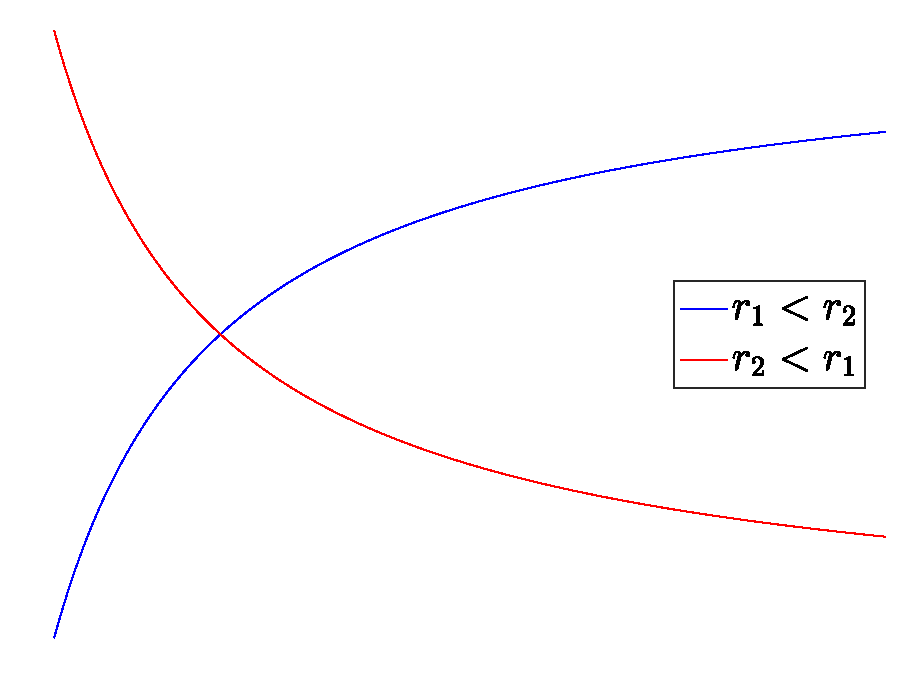
\includegraphics[scale=0.5]{4.35.eps}
    \end{figure}
\end{enumerate}
\clearpage
    \section{合约的套利定价}
\begin{enumerate}[label=\arabic{section}.\arabic*]
    \item \sol
    \begin{enumerate}[label=\alph*)]
        \item $\displaystyle \frac{110-100}{\e^{0.06\times2}}-10=-1.1308$.
        \item $\displaystyle \frac{0}{\e^{0.06\times2}}-10=-10$.
    \end{enumerate}
    \item \sol
    \begin{enumerate}[label=\alph*)]
        \item $\displaystyle \frac{0}{\e^{0.06\times1/2}}-5=-5$.
        \item $\displaystyle \frac{100-98}{\e^{0.06\times1/2}}-5=-3.059$.
    \end{enumerate}
    \item \sol\\
    利用一价律,有\[S=K\e^{-r}-C \Rightarrow C=S-K\e^{-r}.\]
    \item \pro\\
    若$C>S$,则通过同时卖出看涨期权和购买证券来实现套利.
    \item \sol\\
    由命题5.2.2,有$S+P-C=K\e^{-rt}$,而$P \geq 0$,所以$K\e^{-rt} \geq S-C$.
    \item \sol\\
    由上一题,$C \geq S-K\e^{-rt}=30-28\e^{-0.05/3}=2.4628$.
    \item \sol\\
    由练习5.4,有$C \leq S$,则
    \begin{enumerate}[label=\alph*)]
        \item $P-S=K\e^{-rt}+C-2S$,正负皆有可能,该式不一定成立.
        \item $P-K\e^{-rt}=C-S \leq 0 \Rightarrow P \leq K\e^{-rt} \leq K$,该式一定成立.
    \end{enumerate}
    \item \pro \[P-K\e^{-rt}+S=C \geq 0 \Rightarrow P \geq K\e^{-rt}-S.\]
    \item \pro\\
    在时刻0,卖出一股股票$S$,卖出一个看跌期权$P$,买入一个看涨期权$C$,收入$S+P-C$;\\
    在时刻$t$,若$S(t) \leq K$,卖出的看跌期权无用,看涨期权被执行,以执行价$K$买入股票;若$S(t) > K$,买入的看涨期权无用,看跌期权被执行,以执行价$K$买入股票.\\
    由于$S+P-C>K\e^{-rt}$,所以$(S+P-C)\e^{rt}-K>0$,即总可以获得正的收益.
    \item \pro
    \begin{itemize}
        \item 在时刻0,买入一股股票$S$,买入一个看跌期权$P$,卖出一个看涨期权$C$,支出$S+P-C$;在时刻$t$,总是收入$K$.
        \item 向银行存入$K\e^{-rt}$,支出$K\e^{-rt}$,收入$K$.
    \end{itemize}
    所以$S+P-C=K\e^{-rt}$.
    \item \sol\\
    设$P$为看跌期权的价格,则
    \begin{enumerate}[label=\alph*)]
        \item 在时刻0,买入看跌期权$P$、证券$s$;在时刻$t$,由于$K>s_1>s_2$,所以卖出看跌期权$K$,所以回报是$K-(P-S)\e^{rt}$.
        \item $K-(P-S)\e^{rt} 0 \Rightarrow P = K\e^{-rt} - s$.
    \end{enumerate}
    \item \sol
    \begin{itemize}
        \item 在时刻0,买入看涨和看跌期权$P$,支出$C_1+C_2$;在时刻1,收入1.
        \item 向银行存入$\e^{-rt}$,支出$\e^{-rt}$,收入1.
    \end{itemize}
    所以$C_1+C_2=\e^{-rt}$.
    \item \sol\\
    因为$25=S+P-C > K\e^{-rt}=20\e^{-0.1/4}$,所以套利策略为在时刻0,卖出证券$S$,卖出看跌期权$P$,买入看涨期权$C$;在时刻$t$,收入$K$. 回报为$(S+P-C)\e^{rt}-K=5.6329$.
    \item \sol\\
    若这些期权均为欧式期权,令其价格分别为$C,P$,则有\[C_a = C, P_a \geq P,\]
    所以\[S+P-C=K\e^{-rt} \Rightarrow S+P_a-C_a \geq K\e^{-rt}.\]
    \item \pro\\
    若$K_1-K_2 < P_1-P_2$,即$K_2-K_1+P_1-P_2>0$,不妨假设$P_1 > P_2$,在时刻0,卖出$(K_1,P_1)$,买入$(K_2,P_2)$,收入$P_1-P_2$;在时刻$t$,若两者均执行,则支出$K_2-K_1$,则$K_2-K_1+P_1-P_2>0$,存在套利机会,产生矛盾,于是$K_1-K_2 \geq P_1-P_2$.
    \item \sol\\
    设某一美式看跌期权$t$时刻的价格为$P_1$,另一个美式看跌期权$s(s<t)$时刻的价格为$P_2$,即证$P_1 \geq P_2$.\\
    若$P_1 < P_2$,买入$(P_1,t)$,卖出$(P_2,s)$,若两者均执行,则此时收入支出相互抵消,获得初始收益$P_2-P_1$,于是存在套利机会,产生矛盾,所以$P_1 \geq P_2$.
    \item \sol
    \begin{enumerate}[label=\alph*)]
        \item 正确,因为$C=S+P-K\e^{-rt}$关于$t$非减,同时该结论对美式看涨期权也成立.
        \item 错误,因为$F=S\e^{(r_u-r_g)t}$,若要关于$t$非减,需要$r_u \geq r_g$,而题中未说明大小关系.
        \item 错误,因为$P=K\e^{-rt}+C-S$关于$t$非增.
    \end{enumerate}
    \item \sol\\
    设欧式看涨期权的价格为$C$,欧式看跌期权的价格为$P$,则$K=S+P-C$
    \begin{enumerate}[label=\alph*)]
        \item 因为$S+P-C - K\e^{-rt}=(S+P-C)(1-\e^{-rt})>0$,回报为$(S+P-C)\e^{rt}-K=(S+P-C)\e^{rt}-(S+P-C)=(S+P-C)(\e^{rt}-1)>0$,所以这个投资策略恒合理.
        \item 函数是$f(C)=(S+P-C)(\e^{r/4}-1)$,图如下:
        \begin{figure}[H]
            \centering
            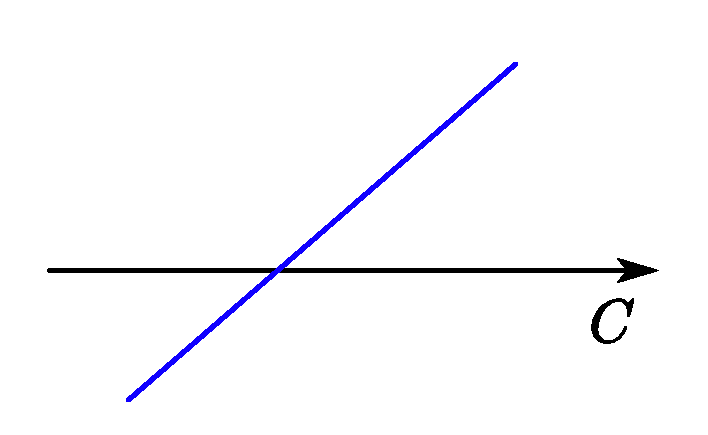
\includegraphics[scale=0.4]{5.18.pdf}
        \end{figure}
    \end{enumerate}
    \item \sol\\ $s-d$.
    \item \sol
    \begin{enumerate}[label=\alph*)]
        \item $(S(t)-K)^++(K-S(t))^+=|S(t)-K|$.
        \item $(S(t)-K_1)^+-(K_2-S(t))^+$.
        \item $2(S(t)-K)^+-S(t)$.
        \item $S(t)-(S(t)-K)^+$.
    \end{enumerate}
    \item \pro\\
    有$C(K)=S+P-K\e^{-rt}$,有$C'(K)=-\e^{-rt}<0$,所以一个欧式看涨期权的价格关于其敲定价是非增的.
    \item \sol
    \begin{enumerate}[label=\alph*)]
        \item $100-105=-5<0$,这个投资的初始成本是负的.
        \item 回报为$f[S(t)]=(S(t)-100)^+-(S(t)-105)^+$,图如下:
        \begin{figure}[H]
            \centering
            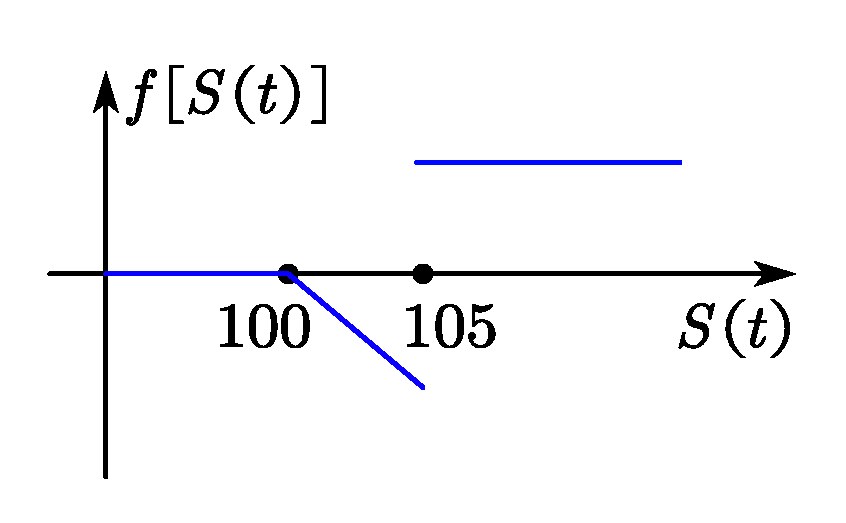
\includegraphics[scale=0.3]{5.22.pdf}
        \end{figure}
    \end{enumerate}
    \item \sol\\
    在时刻0,买入敲定价为110的看涨期权,卖出敲定价为100的看涨期权,收入$20-C$;在时刻$t$,两个看涨期权都执行时,最多支出10,所以$20-C \leq 10\e^{-rt}$,即$C \geq 20-10\e^{-rt}$.
    \item \pro\\ 因为$S+P-C=K\e^{-rt}$,所以$P(K,t)=K\e^{-rt}+C-S$,显然$P(K,t)$对于固定的$t$,关于$K$是凸函数(也是凹函数).
    \item \sol\\ 可以,考虑两个投资
    \begin{itemize}
        \item 购买1份$(K,t)$美式看跌期权;
        \item 购买$\lambda$份$(K_1,t)$美式看跌期权和$(1-\lambda)$份$(K_2,,t)$美式看跌期权.
    \end{itemize}
    其中$K=\lambda K_1+(1-\lambda)K_2$. 当证券价格为$s$时,回报为$(K^*-s)^+$,$K^*$为看跌期权的执行价. 根据回报的凸性,即可得价格的凸性.
    \item \pro\\
    若$t_1$时刻期权价格是$s$,在此时卖出证券,收入$s-K_1$;在$t_2$时刻买回证券,等价于$t_1$时刻收入$s-K_2\e^{-r(t_2-t_1)}$. 因为$K_1>K_2\e^{-r(t_2-t_1)}$,所以$t_1$时刻不会执行该期权.
    \item \pro\\
    由于$-\max\{a,b\}=\min\{-a,-b\}$,则
    \[S(t)-\max\{K,S(t)-A\}=S(t)+\min\{-K,-S(t)+A\}=\min\{S(t)-K,A\},\]
    所以\[(S(t)-\max\{K,S(t)-A\})^+=\max\{0,\min\{S(t)-K,A\}\}=\min\{(S(t)-K)^+,A\}.\]
    \item \omitted
    \item \sol
    \begin{enumerate}[label=\alph*)]
        \item 几何解释:原曲线上任意两点形成的弦上的端(不含端点)都在原曲线下方,图如下:
        \begin{figure}[H]
            \centering
            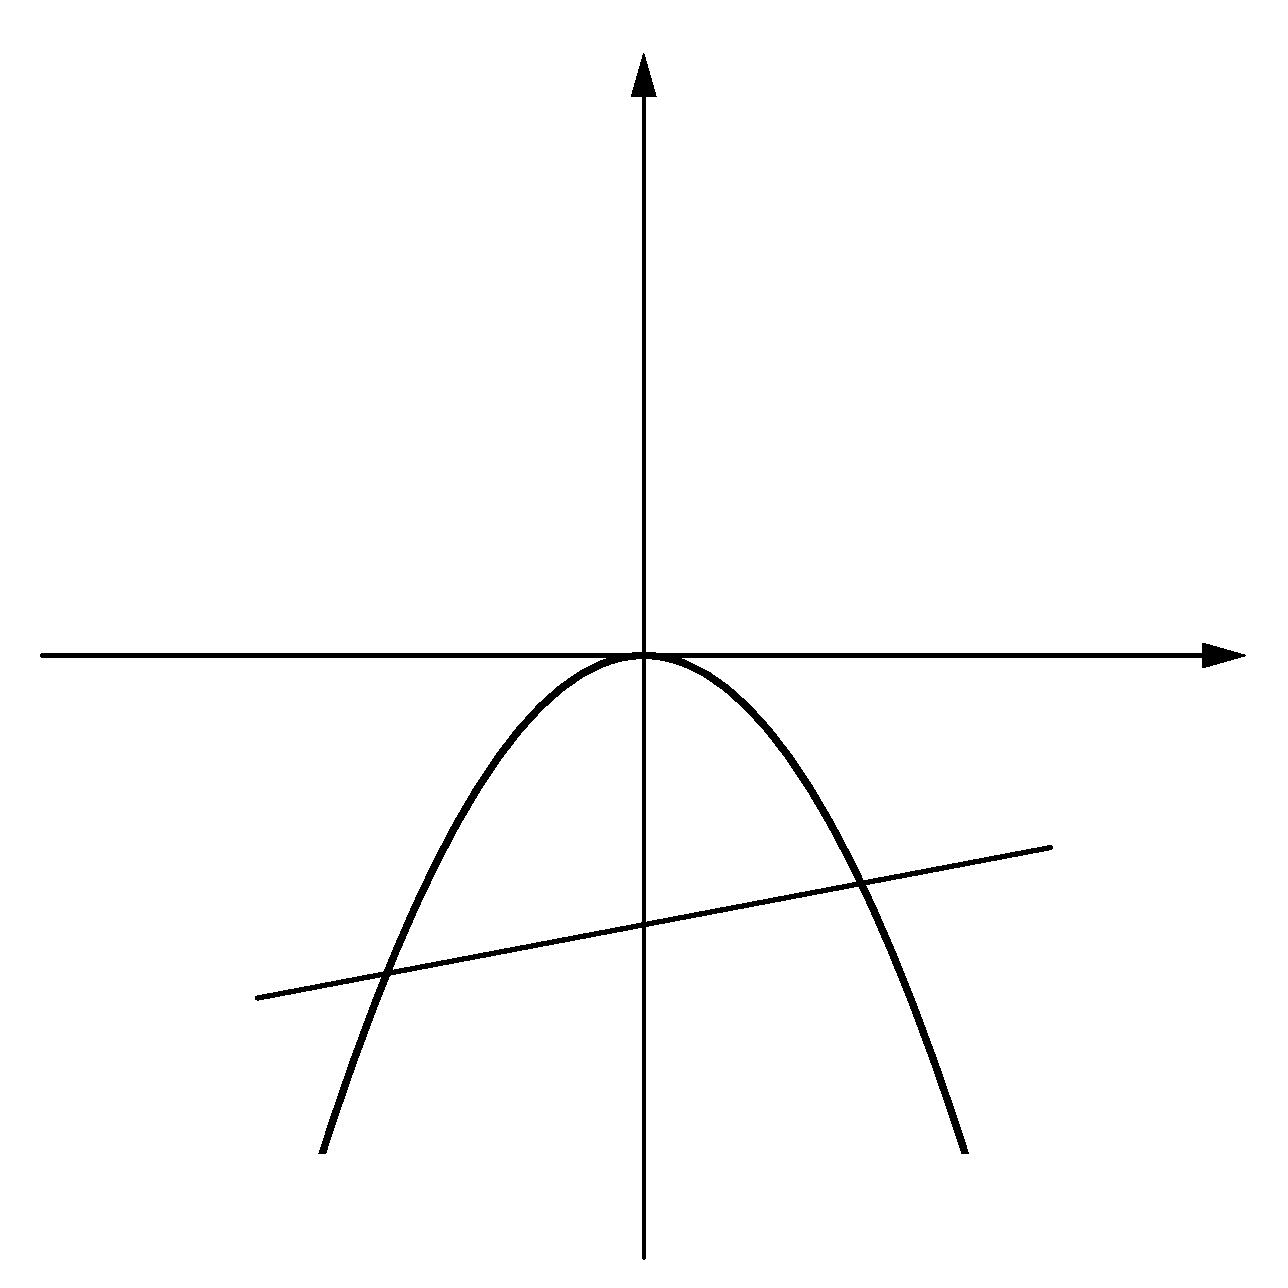
\includegraphics[scale=0.2]{5.28.pdf}
        \end{figure}
        \item \begin{align*}
            f(x)\text{是凹函数} & \iff f[\lambda x+(1-\lambda)y] \geq \lambda f(x)+(1-\lambda)f(y)\\
            &\iff -f[\lambda x+(1-\lambda)y] \leq -\lambda f(x)-(1-\lambda)f(y)\\
            & \iff g[\lambda x+(1-\lambda)y] \leq \lambda g(x)+(1-\lambda)g(y)\\
            &\iff g(x)\text{是凸函数}
        \end{align*}
    \end{enumerate}
    \item \sol
    \begin{enumerate}[label=\alph*)]
        \item $E(X_1) < E(X_2)$无法说明一定能获利,故无法说明存在套利.
        \item $P(X_2>X_1)>0$无法说明一定能获利,故无法说明存在套利.
    \end{enumerate}
\end{enumerate}
\clearpage
    \section{套利定理}
\begin{enumerate}[label=\arabic{section}.\arabic*]
    \item \sol\\
    不存在. 因为$\displaystyle p_i=\frac{1}{1+o_i}$,即
    \[p_1=\frac{1}{2},p_2=\frac{1}{3},p_3=\frac{1}{6} \Rightarrow \sum_{i=1}^3 p_i=1,\]
    所以不存在一个稳赢的赌博策略.
    \item \sol \[\frac{1}{1+2}+\frac{1}{1+3}+\frac{1}{1+o_4}=1 \Rightarrow o_4=\frac{47}{13}.\]
    \item \sol
    \begin{enumerate}[label=\alph*)]
        \item \[\begin{cases}
            4p_1+8p_2-10p_3=0,\\6p_1+12p_2-16p_3=0,
        \end{cases} \Rightarrow \rank \left(\begin{array}{ccc}
            \begin{matrix}
                4 & 8 & -10\\6 & 12 & -16
            \end{matrix}
        \end{array}\right)=2 \Rightarrow \text{不存在满足条件的}p_i,\]
        所以存在套利.
        \item \[\begin{cases}
            6p_1-3p_2=0,\\-2p_1+6p_3=0,\\10p_1+10p_2+xp_3=0,
        \end{cases} \text{有解} \Rightarrow x=-90,p_1=0.3,p_2=0.6,p_3=0.1,\]
        所以没有套利时,$x=-90$.
    \end{enumerate}
    \item \sol\\
    不存在套利时,仍有$\displaystyle p_1=\frac{1}{2},p_2=\frac{1}{3},p_3=\frac{1}{6}$,则
    \[\begin{cases}
        o_{12}(p_1+p_2)-p_3=0,\\o_{23}(p_2+p_3)-p_1=0,\\o_{13}(p_1+p_3)-p_2=0
    \end{cases} \Rightarrow \begin{cases}
        o_{12}=\frac{1}{5}, \\ o_{23}=1, \\ o_{13}=\frac{1}{2}.
    \end{cases}\]
    \item \pro\\
    若结果是$j$,则
    \begin{align*}
        o_jx_j-\sum_{i \neq j}x_i & = o_jx_j-\sum_{i = 1}^m x_i+x_j=(1+o_j)x_j-\sum_{i = 1}^m x_i\\
        &=\frac{(1+o_j)(1+o_j)^{-1}-\sum\limits_{i=1}^m (1+o_i)^{-1}}{1-\sum\limits_{i=1}^m (1+o_i)^{-1}}=1
    \end{align*}
    \item \sol\\
    购买看跌期权的收益为
    \[\begin{cases}
        -P, & \text{价格为}200 \\ \displaystyle\frac{100}{1+r}-P, & \text{价格为}50
    \end{cases}\]
    则\[E(\text{收益})=p\times(-P)+(1-p)\times\left(\frac{100}{1+r}-P\right)=(1-p)\frac{100}{1+r}-P,\]
    所以$\displaystyle P=(1-p)\frac{100}{1+r}=\left(1-\frac{1+2r}{3}\right)\frac{100}{1+r}=\frac{200(1-r)}{3(1+r)}$.\\
    因为$\displaystyle S+P-C=\frac{K}{1+r} \Rightarrow C=S+P-\frac{K}{1+r}$,代入可验证其成立.
    \item \sol\\
    先计算$\displaystyle p=\frac{1+r-d}{u-d}=\frac{1-1/2}{2-1/2}=\frac{1}{3}$(其中$r=0$),则有
    \begin{figure}[H]
        \centering
        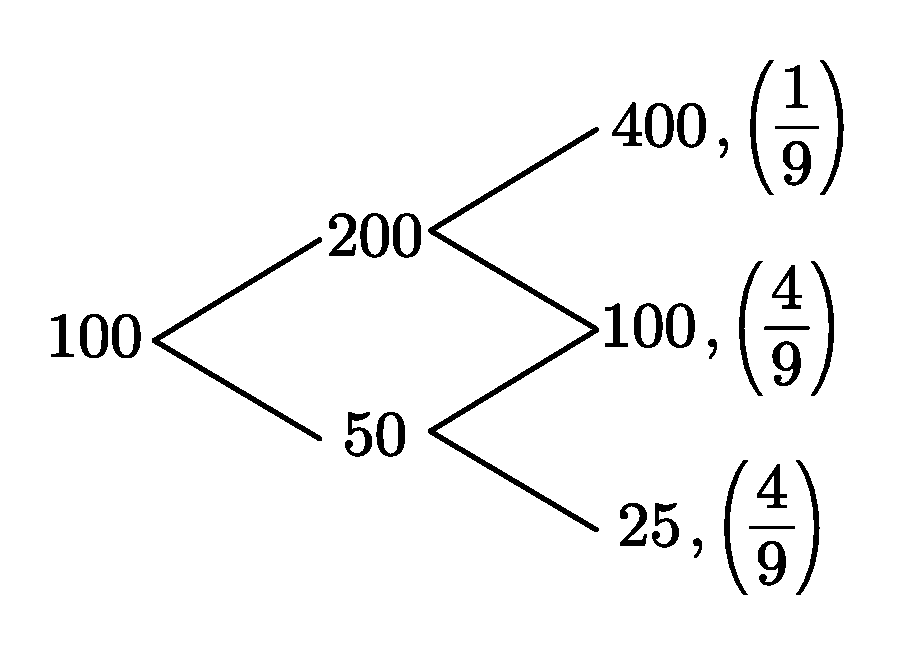
\includegraphics[scale=0.3]{6.7.pdf}
    \end{figure}
    所以收益为\[\begin{cases}
        \displaystyle\frac{250}{(1+r)^2}-C, & \text{概率为}1/9 \\ -C, & \text{概率为}4/9 \\ -C, & \text{概率为}4/9
    \end{cases}\]
    要使期望收益为0,则
    \[E(\text{收益})=\frac{250-C}{9}-\frac{4}{9}C-\frac{4}{9}C=0 \Rightarrow C=\frac{250}{9}.\]
    \item \sol {\kaishu \textcolor{blue}{注意:也可以参照教材例9.1a的解法.}}\\
    \begin{figure}[H]
        \centering
        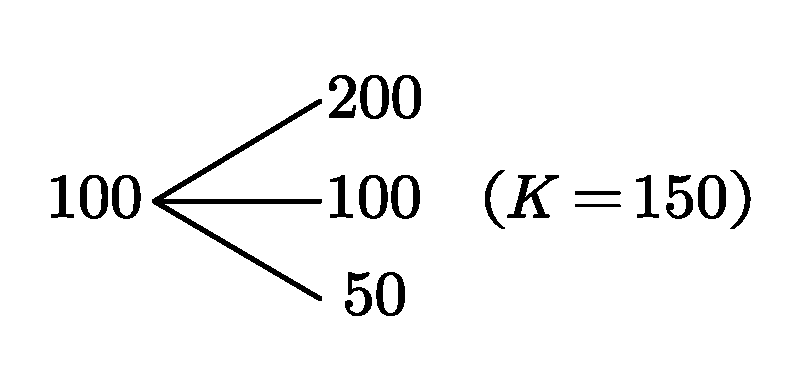
\includegraphics[scale=0.35]{6.8.pdf}
    \end{figure}
    买入股票的收益为
    \[\begin{cases}
        \displaystyle\frac{200}{1+r}-100, & \text{概率为}p_1 \\ \displaystyle\frac{100}{1+r}-100, & \text{概率为}p_2 \\ \displaystyle\frac{50}{1+r}-100, & \text{概率为}p_3 \\
    \end{cases}\]
    所以
    \[E(\text{买入股票的收益})=\left(\frac{200}{1+r}-100\right)p_1+\left(\frac{100}{1+r}-100\right)p_2+\left(\frac{50}{1+r}-100\right)p_3=0,\]
    买入期权的收益为$\displaystyle \begin{cases}
        \displaystyle\frac{50}{1+r}-C, & \text{概率为}p_1 \\ -C, & \text{概率为}p_2 \\ -C, & \text{概率为}p_3 \\
    \end{cases}$,所以\[E(\text{买入期权的收益})=\left(\frac{50}{1+r}-C\right)p_1-Cp_2-Cp_3=0,\]
    由后式可得$\displaystyle C=\frac{50p_1}{1+r}$,由前式可得
    \begin{align*}
        &\left(\frac{200}{1+r}\right)p_1+\left(\frac{100}{1+r}\right)p_2+\left(\frac{50}{1+r}\right)p_3=100(p_1+p_2+p_3)=100\\
        \Rightarrow & 2p_1+p_2+\frac{1}{2}p_3=1+r \Rightarrow 2p_1+p_2+\frac{1}{2}(1-p_1-p_2)=1+r\\
        \Rightarrow & 3p_1+p_2=1+2r \Rightarrow p_1=\frac{1+2r-p_2}{3}
    \end{align*}
    所以$\displaystyle C=\frac{50p_1}{1+r}=\frac{1+2r-p_2}{3}\cdot\frac{50}{1+r}$,由$0 \leq p_2 \leq 1$可得
    \[\frac{2r}{3}\cdot\frac{50}{1+r} \leq C \leq \frac{1+2r}{3}\cdot\frac{50}{1+r} \Rightarrow 0 \leq C \leq \frac{50}{3}.\]
    \item \sol
    \begin{enumerate}[label=\alph*)]
        \item 若$C=0$,则在时刻0,无支出;在时刻1可收入50或0,这显然是个弱套利.
        \item 若$\displaystyle C=\frac{50}{3}$,则在时刻0,卖出一个看涨期权,并买入$x$股股票;在时刻1,收入如下表:
        \begin{table}[H]
            \centering
            \begin{tabular}{|c|c|c|c|}
                \hline
                时刻1股票的价格 & 时刻0的余额 & 时刻1该投资的现值 & 收入$(r=0)$ \\ \hline
                200 & $50/3-100x$ & $-50+200x$ & $100x-100/3$ \\ \hline
                100 & $50/3-100x$ & $0+100x$ & $50/3$ \\ \hline
                50 & $50/3-100x$ & $0+50x$ & $-50x-100/3$ \\ \hline
            \end{tabular}
        \end{table}
        若$\displaystyle x=\frac{1}{3}$,则显然存在弱套利机会. 综上,弱套利可能存在.
    \end{enumerate}
    \item \sol\\
    令$S(0)=s$,假设$us>K>ds$. 如果通过借$x$来买入$y$份证券,则在时刻$t$,剩余$ys-x$的收入为
    \[\begin{cases}
        yus-(1+r)x, & S(1)=us\\yds-(1+r)x, & S(1)=ds
    \end{cases}\]
    所以可以通过如下方式复制期权,
    \[\begin{cases}
        yus-(1+r)x=us-K,\\yds-(1+r)x=0,
    \end{cases}\]
    令$\displaystyle y=\frac{us-K}{(u-d)s},x=\frac{ds(us-K)}{(1+r)(u-d)s}$,则根据一价律,期权的无套利价格是$\displaystyle ys-x=\frac{us-K}{u-d}-\frac{ds(us-K)}{(1+r)(u-d)s}$.
    \item \sol
    \begin{enumerate}[label=\alph*)]
        \item $\displaystyle p=\frac{1+r-d}{u-d}=\frac{0.3}{0.425}=\frac{12}{17}$,期望收益为$25(1-p)^2p^3=0.7606$,所以无套利价格是$0.7606\times 1.1^{-5}=0.4723$.
        \item 是唯一的. 证明略.
        \item $\displaystyle 25 \times \left(\frac{1}{2}\right)^5=0.78125$.
    \end{enumerate}
    \item \sol\\
    $\displaystyle p=\frac{1+r-d}{u-d}=0.7380$,如果前3个时刻中至少有2个时刻是向上的,则可得到回报,所以
    \[C=\e^{-0.05 \times 3}\times 100 \left[0.7380^3+3(0.7380)^2(1-0.7380)\right]=84.5228.\]
\end{enumerate}
\clearpage
    \section{Black-Scholes公式}
\begin{enumerate}[label=\arabic{section}.\arabic*]
    \item \sol\\
    因为$\displaystyle \ln\left(\frac{S(t)}{S(0)}\right) \sim N\left(\left(r-\frac{\sigma^2}{2}\right)t,\sigma^2t\right)$,所以$\displaystyle \ln\left(\frac{S(t_1)}{S(t_2)}\right) \sim N\left(\left(r-\frac{\sigma^2}{2}\right)(t_1-t_2),\sigma^2(t_1-t_2)\right)$.
    \begin{enumerate}[label=\alph*)]
        \item $\displaystyle \sigma_d=0.33\sqrt{\frac{n-(n-1)}{365}}=0.0173$.
        \item $\displaystyle \sigma_m=0.33\sqrt{\frac{n-(n-1)}{12}}=0.0953$.
    \end{enumerate}
    \item \sol\\
    $\displaystyle t=\frac{4}{12}=\frac{1}{3}$,所以期权被执行当且仅当$\displaystyle S\left(\frac{1}{3}\right)>42$,而$\displaystyle \ln\frac{S(1/3)}{S(0)} \sim N\left(0.04,0.0192\right)$则
    \begin{align*}
        P\left[S\left(\frac{1}{3}\right)>42\right]&=P\left[\frac{S(1/3)}{S(0)}>\frac{42}{40}\right]=P\left[\ln\frac{S(1/3)}{S(0)}>\ln1.05\right]\\
        &=P\left(Z>\frac{\ln1.05-0.04}{\sqrt{0.0192}}\right)=1-\Phi(0.0634)\\
        &=1-0.5253=0.4747
    \end{align*}
    \item \sol\\
    本题中的参数为\[t=\frac{1}{3},r=0.08,\sigma=0.24,K=42,S(0)=40,\]
    则\[\omega=\frac{rt+\sigma^2t/2-\ln[K/S(0)]}{\sigma\sqrt{t}}=\frac{0.08/3+0.24^2/6-\ln(42/40)}{0.24/\sqrt{3}}=-0.0904,\]
    而$\Phi(-0.0904)=0.4640,\Phi(-0.2290)=0.4094$,所以
    \[C=S(0)\Phi(\omega)-K\e^{-rt}\Phi(\omega-\sigma\sqrt{t})=40\times0.4640-42\e^{-0.08/3}\times0.4094=1.8177.\]
    \item \sol\\
    由看跌-看涨期权平价公式,则
    \begin{align*}
        P&=C-S(0)+K\e^{-rt}=S(0)\Phi(\omega)-K\e^{-rt}\Phi(\omega-\sigma\sqrt{t})-S(0)+K\e^{-rt}\\
        &=S(0)[\Phi(\omega)-1]+K\e^{-rt}[1-\Phi(\omega-\sigma\sqrt{t})]
    \end{align*}
    本题中的参数为\[t=\frac{1}{2},r=0.10,\sigma=0.30,K=100,S(0)=105,\]
    则\[\omega=\frac{rt+\sigma^2t/2-\ln[K/S(0)]}{\sigma\sqrt{t}}=\frac{0.1/2+0.3^2/4-\ln(100/105)}{0.3/\sqrt{2}}=0.5718,\]
    而$\Phi(0.5718)=0.7163,\Phi(0.3596)=0.6404$,所以
    \[P=105\times(0.7163-1)+100\e^{-0.1/2}\times(1-0.6404)=4.4177.\]
    \item \sol {\kaishu \textcolor{blue}{注意:b)问少了一个条件:假设$r=0.05$.}}
    \begin{enumerate}[label=\alph*)]
        \item \begin{align*}
            P\left[\frac{S(0.5)}{S(0)}<0.9\right]&=P\left[\ln\frac{S(0.5)}{S(0)}<\ln0.9\right]=P\left(Z<\frac{\ln0.9-0.03}{\sqrt{0.3^2\times0.5}}\right)\\
            &=\Phi(-0.6381)=1-\Phi(0.6381)=1-0.7383=0.2617
        \end{align*}
        \item $\displaystyle r-\sigma^2/2=0.05-0.045=0.005$,与a)问类似,
        \begin{align*}
            P\left[\frac{S(0.5)}{S(0)}<0.9\right]&=P\left[\ln\frac{S(0.5)}{S(0)}<\ln0.9\right]=P\left(Z<\frac{\ln0.9-0.0025}{\sqrt{0.3^2\times0.5}}\right)\\
            &=\Phi(-0.5085)=1-\Phi(0.5085)=1-0.7383=0.3056
        \end{align*}
        投资的收益为\[\begin{cases}
            100\e^{-rt}-A, & \text{概率为}0.3056 \\ -A, & \text{概率为}0.7383
        \end{cases}\]
        所以\[E(\text{收益})=0.3056(100\e^{-0.025}-A)-0.7383A=0 \Rightarrow A=29.8055.\]
    \end{enumerate}
    \item \sol
    \begin{enumerate}[label=\alph*)]
        \item 本题中的参数为\[t=\frac{1}{4},r=0.04,\sigma=0.3,K=100,S(0)=95,\]
        则\[\omega=\frac{rt+\sigma^2t/2-\ln[K/S(0)]}{\sigma\sqrt{t}}=\frac{0.04/4+0.3^2/8-\ln(100/95)}{0.3/\sqrt{4}}=-0.2003,\]
        而$\Phi(-0.2003)=0.4206,\Phi(-0.3503)=0.3631$,所以
        \[C=S(0)\Phi(\omega)-K\e^{-rt}\Phi(\omega-\sigma\sqrt{t})=95\times0.4206-100\e^{-0.04/4}\times0.3631=4.0083.\]
        \item \begin{align*}
            P[S(1/4)<100]&=P\left[\frac{S(1.4)}{S(0)}<\frac{100}{95}\right]=P\left[\ln\frac{S(1.4)}{S(0)}<\ln\frac{100}{95}\right]\\
            &=P\left(Z<\frac{\ln(100/95)-0.05/4}{\sqrt{0.3^2/4}}\right)\\
            &=\Phi(0.2586)=0.6020
        \end{align*}
        \item $\displaystyle r-\frac{\sigma^2}{2}=-0.005$,下计算$P[S(1)>105]$,
        \[P[S(1)>105]=P\left(Z>\frac{\ln(105/95)+0.005}{0.3}\right)=1-\Phi(0.3503)=0.3631,\]
        再计算$P[S(1)>S(0.5)]$,\[P[S(1)>S(0.5)]=P\left(Z>\frac{0+0.005/2}{0.3/\sqrt{2}}\right)=1-\Phi(0.0118)=0.4953,\]
        则$0.3631 \times 0.4953=0.1798$,而收益为
        \[\begin{cases}
            50\e^{-rt}-C, & \text{概率为}0.1798\\-C, & \text{概率为}1-0.1798
        \end{cases}\]
        所以\[E(\text{收益})=0.1798(50\e^{-0.04}-C)-(1-0.1798)C=0 \Rightarrow C=0.1798\times50\e^{-0.04}=8.6375.\]
    \end{enumerate}
    \item \sol\\
    本题中的参数为\[t=\frac{1}{2},r=0.06,\sigma=0.32,K=40,S(0)=38,F=100,\]
    $\displaystyle r-\frac{\sigma^2}{2}=0.0088$,下计算$P[S(1/2)>K]$,
    \[P[S(1/2)>K]=P\left(Z>\frac{\ln(40/38)-0.0088/2}{\sqrt{0.32^2/2}}\right)=1-\Phi(0.2072)=0.4179,\]
    收益为
    \[\begin{cases}
        F\e^{-rt}-C, & \text{概率为}0.4179\\-C, & \text{概率为}1-0.4179
    \end{cases}\]
    所以
    \[E(\text{收益})=0.4179(100\e^{-0.06/2}-C)-(1-0.4179)C=0 \Rightarrow C=0.4179\times100\e^{-0.03}=40.5549.\]
    \item \sol\\
    本题中的参数为\[t=\frac{1}{2},r=0.06,\sigma=0.32,K=40,S(0)=38,F=100,\mu=0,\]
    $\displaystyle r-\frac{\sigma^2}{2}=0.0088$,下计算$P[S(1/2)>K]$
    \[P[S(1/2)>K]=P\left(Z>\frac{\ln(40/38)-0}{\sqrt{0.32^2/2}}\right)=1-\Phi(0.2267)=0.4179,\]
    收益为
    \[\begin{cases}
        F\e^{-rt}-C, & \text{概率为}0.4103\\-C, & \text{概率为}1-0.4103
    \end{cases}\]
    所以
    \[E(\text{收益})=0.4103(100\e^{-0.06/2}-C)-(1-0.4103)C=0 \Rightarrow C=0.4103\times100\e^{-0.03}=39.8174.\]
    \item \sol\\ 否,还需要知道几何布朗运动的漂移参数$\mu$.
    \item \sol
    \begin{enumerate}[label=\alph*)]
        \item $\displaystyle r-\frac{\sigma^2}{2}=-0.02$,下计算$P[S(1)<95]$,
        \[P[S(1)<95]=P\left(Z<\frac{\ln(95/100)+0.02}{\sqrt{0.4^2}}\right)=\Phi(-0.0782)=0.4688,\]
        再计算$P[S(1)>110]$,
        \[P[S(1)>110]=P\left(Z>\frac{\ln(110/100)+0.02}{\sqrt{0.4^2}}\right)=1-\Phi(0.2883)=0.3866,\]
        收益为
        \[\begin{cases}
            5\e^{-rt}-10, & \text{概率为}0.4688\\x\e^{-rt}-10, & \text{概率为}0.3866\\0, & \text{概率为}1-0.4688-0.3866
        \end{cases}\]
        所以
        \[E(\text{收益})=0.4688(5\e^{-0.06}-10)+0.3866(x\e^{-0.06}-10)=0 \Rightarrow x=17.4313.\]
        \item \[P[S(1)<95]=P\left(Z<\frac{\ln(95/100)-0.05}{\sqrt{0.4^2}}\right)=\Phi(-0.2532)=0.4001.\]
    \end{enumerate}
    \item \sol
    \begin{enumerate}[label=\alph*)]
        \item 因为
        \begin{align*}
            P[S(0.5) \geq 42 \cup S(1)>1.05S(0.5)]&=1-P[S(0.5) < 42 \cap S(1) \leq 1.05S(0.5)]\\
            &=1-P[S(0.5) < 42]P[S(1) \leq 1.05S(0.5)]
        \end{align*}
        而$\displaystyle r-\frac{\sigma^2}{2}=-0.02$,下计算$P[S(0.5) \geq 42]$,
        \[P[S(0.5) < 42]=P\left(Z < \frac{\ln(42/40)+0.02/2}{\sqrt{0.4^2/2}}\right)=\Phi(0.2079)=0.5823,\]
        再计算$P[S(1) \leq 1.05S(0.5)]$,
        \[P[S(1) \leq 1.05S(0.5)]=P\left(Z\leq\frac{\ln1.05+0.02/2}{\sqrt{0.4^2/2}}\right)=\Phi(0.2079)=0.5823,\]
        $1-0.5823^2=1-0.3391=0.6609$,收益为
        \[\begin{cases}
            100\e^{-rt}-C, & \text{概率为}0.6609\\-C, & \text{概率为}1-0.6609
        \end{cases}\]
        所以
        \[E(\text{收益})=0.6609(100\e^{-0.06}-C)-(1-0.6609)C=0 \Rightarrow C=0.6609\times100\e^{-0.06}=62.2412.\]
        \item 因为
        \begin{align*}
            P[S(0.5) \geq 42 \cup S(1)>1.05S(0.5)]&=1-P[S(0.5) < 42 \cap S(1) \leq 1.05S(0.5)]\\
            &=1-P[S(0.5) < 42]P[S(1) \leq 1.05S(0.5)]
        \end{align*}
        下计算$P[S(0.5) \geq 42]$,
        \[P[S(0.5) < 42]=P\left(Z < \frac{\ln(42/40)-0.06/2}{\sqrt{0.4^2/2}}\right)=\Phi(0.0664)=0.5265,\]
        再计算$P[S(1) \leq 1.05S(0.5)]$,
        \[P[S(1) \leq 1.05S(0.5)]=P\left(Z\leq\frac{\ln1.05-0.06/2}{\sqrt{0.4^2/2}}\right)=\Phi(0.0664)=0.5265,\]
        所以合约赢利的概率为$1-0.5265^2=0.7288.$
    \end{enumerate}
    \item \sol
    \begin{enumerate}[label=\alph*)]
        \item $\displaystyle r-\frac{\sigma^2}{2}=0$,下计算$P[S(1)>(1+x)40]$,
        \[P[S(1)>(1+x)40]=P\left(Z > \frac{\ln(1+x)-0}{\sqrt{0.2^2}}\right)=1-\Phi[5\ln(1+x)],\]
        收益为
        \[\begin{cases}
            100\e^{-rt}-10, & \text{概率为}1-\Phi[5\ln(1+x)]\\-10, & \text{概率为}\Phi[5\ln(1+x)]
        \end{cases}\]
        所以
        \begin{align*}
            E(\text{收益})=&(1-\Phi[5\ln(1+x)])(100\e^{-0.02}-10)-10\Phi[5\ln(1+x)]=0\\
            \Rightarrow & \Phi[5\ln(1+x)]=0.8980 \Rightarrow x=0.2892.
        \end{align*}
        \item \[P[S(1)>(1+x)40]=P\left(Z > \frac{\ln(1+x)-0.04}{\sqrt{0.2^2}}\right)=1-\Phi[5\ln(1+x)-0.2]=0.1423.\]
    \end{enumerate}
    \item \sol\\
    $C(s,t,K,r,\sigma)=s\Phi(\omega)-K\e^{-rt}\Phi(\omega-\sigma\sqrt{t})$,具体推导见定理7.5.1.
    \item \sol\\
    因为$\max\{0,S(t)-K\}=\max\{0,S(t)-0\}=S(t)$,所以执行价为0的看涨期权等价于一个价格为$S(0)$的股票,所以价格为$S(0)$.
    \item \sol\\
    根据Black-Scholes公式:
    \[C=S(0)\Phi(\omega)-K\e^{-rt}\Phi(\omega-\sigma\sqrt{t}),\]
    其中$\displaystyle \omega=\frac{rt+\sigma^2t/2-\ln[K/S(0)]}{\sigma\sqrt{t}}$,所以当$t \to +\infty$时,$\omega \to +\infty, \omega-\sigma\sqrt{t} \to +\infty$,所以$C \to S(0)$,它的价格会趋向于$S(0)$.
    \item \sol\\
    根据Black-Scholes公式:
    \[C=S(0)\Phi(\omega)-K\e^{-rt}\Phi(\omega-\sigma\sqrt{t}),\]
    其中$\displaystyle \omega=\frac{rt+\sigma^2t/2-\ln[K/S(0)]}{\sigma\sqrt{t}}$,所以当$\sigma \to 0$时,$\omega \to 0, \omega-\sigma\sqrt{t} \to 0$,所以$\displaystyle C \to \frac{S(0)-K\e^{-rt}}{2}$,它的价格会趋向于$\displaystyle \frac{S(0)-K\e^{-rt}}{2}$.
    \item \sol
    \begin{figure}[H]
        \centering
        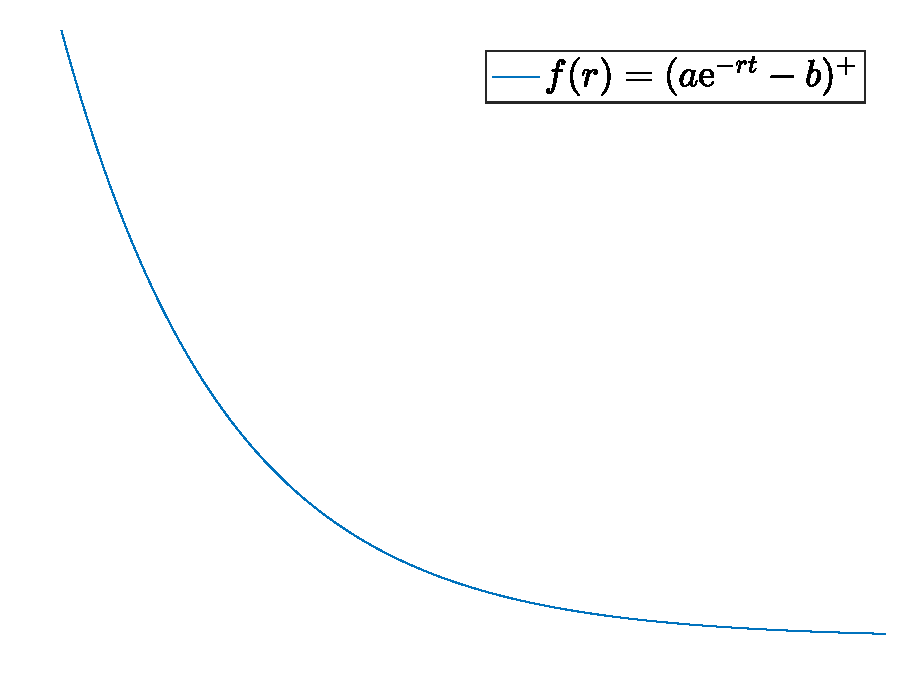
\includegraphics[scale=0.4]{7.17.eps}
    \end{figure}
    \item \sol\\
    没有绝对的凹凸性.
\end{enumerate}
\clearpage
    \section{关于期权的其他结果}
\begin{enumerate}[label=\arabic{section}.\arabic*]
    \item \sol\\ 成立.
    \item \sol\\ 服从一个漂移参数为$\displaystyle r-\frac{\sigma^2}{2}-f$,波动参数为$\sigma$的几何布朗运动.
    \item \sol\\ $C(s(1-f)^2,K,t,r,\sigma)$.
    \item \pro\\ 在没有分红时,不应该提前执行看涨期权,所以不应该在$t_d$之前或在$(t_d, t)$之间执行看涨期权,即所证.
    \item \sol\\ 上限期权的收益是$(K,t)$看涨期权和$(K+B,t)$看涨期权收益的差,因此,根据一价律,无套利价格为$C(s,K, t, r, \sigma) - C(s,K + B, t, r, \sigma)$.
    \item \sol\\ 在风险中性几何布朗运动下,该投资的预期收益为
    \[E[(1+\beta)s+\alpha(S(1)-(1+\beta)s)^+]=(1+\beta)s+\alpha\e^{r}C(s,t,(1+\beta)s,\sigma,r),\]
    由于无套利存在,所以上式等于$s\e^r$,可解得
    \[\alpha=\frac{s(\e^r-1-\beta)}{\e^rC(s,t,(1+\beta)s,\sigma,r)}.\]
    \item \pro\\ 在风险中性几何布朗运动下,当$K>(1+\beta)s$时,该投资的预期收益为
    \[E[(1+\beta)s+(S(1)-(1+\beta)s)^+-(S(1)-K)^+] = (1+\beta)s+\e^rC(s, t, (1+\beta)s, \sigma, r)-\e^rC(s, t,K, \sigma, r),\]
    由于无套利存在,所以上式等于$s\e^r$,化简即可得
    \[C(s, 1,K, \sigma, r)=C(s, 1, s(1+\beta), \sigma, r)+s(1+\beta)\e^{-r}-s.\]
    同时,因为$s(1+\beta)\e^{-r}-s<0$,而$C(s, t,K, \sigma, r)$关于$K$递减,所以$K>(1+\beta)s$一定成立,即上式必成立.
    \item \pro \begin{align*}
        C(s\e^{-ft},t,K,\sigma,r)&=\e^{-rt}E[(s\e^{-ft}\e^W-K)^+]=\e^{-rt}E[(s\e^{-ft}\e^{\sigma\sqrt{t}Z+(r-\sigma^2/2)t}-K)^+]\\
        &=\e^{-rt}E[(s\e^{\sigma\sqrt{t}Z+(r-f-\sigma^2/2)t}-K)^+]\\
        &=\e^{-rt}\e^{-(r-f)t}E[(s\e^{\sigma\sqrt{t}Z+(r-f-\sigma^2/2)t}-K)^+]\\
        &=\e^{-rt}C(s,t,K,\sigma,r-f)
    \end{align*}
    \item \pro
    \begin{enumerate}[label=\alph*)]
        \item 比起在时刻$s<t_1$执行看涨期权支付$K_1$,显然在时刻$t_1$执行看涨期权支付$K_1$会更好.
        \item 因为在时刻$t_1$,看涨期权的价格为$C(x,t-t_1,K,\sigma,r)$,同时$S(t_1)=x$.
        \item 因为$C(y,t-t_1,K,\sigma,r)$关于$y$严格单调递增.
        \item 因为在时刻$t_1$行使购买看涨期权的期权是最佳策略当且仅当$S(t_1) \geq x$.
    \end{enumerate}
    \item \pro
    \begin{enumerate}[label=\alph*)]
        \item 若在时刻$t_2$执行期权,支付$K_2\e^{-rt_2}$;若在时刻$t_1$执行期权,支付$K_1\e^{-rt_1}$. 因为$K_1>\e^{-r(t_2-t_1)}K_2 \Rightarrow K_2\e^{-rt_2}<K_1\e^{-rt_1}$,所以不应该在时刻$t_1$执行期权.
        \item 若在时刻$t_1$期权不执行且$S(t_1)=y$,此时的风险中性收益为$C(y,t_2-t_1,K_2,\sigma,r)$. 若在时刻$t_1$期权执行,此时的收益为$y-K_1$. 所以当$S(t_1)=y$时,若$C(y,t_2-t_1,K_2,\sigma,r)<y-K_1$则应该在时刻$t_1$执行期权,证毕.
    \end{enumerate}
    \item \sol
    \begin{figure}[H]
        \centering
        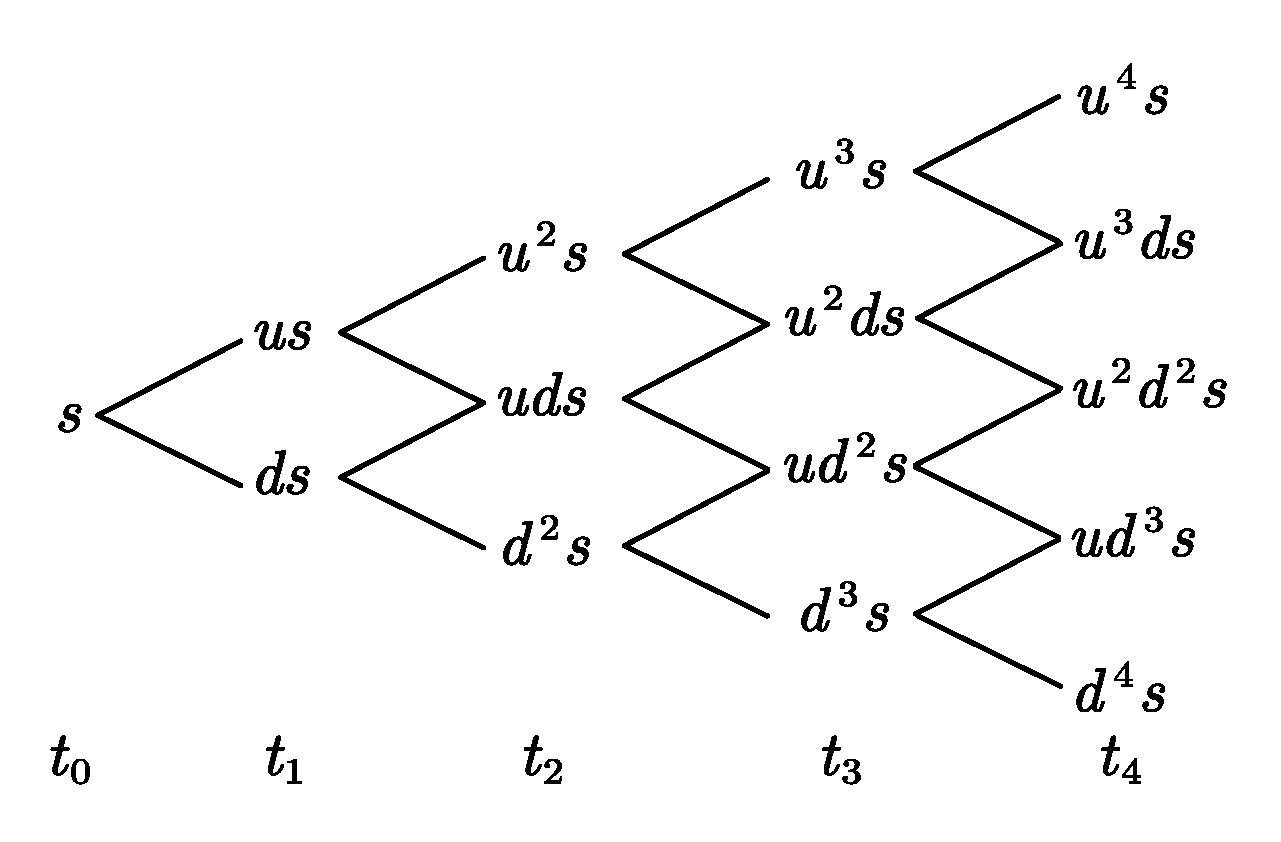
\includegraphics[scale=0.35]{8.11.pdf}
    \end{figure}
    \item \sol
    \begin{enumerate}[label=\alph*)]
        \item 正确,原因略.
        \item 错误,原因略.
        \item 错误,原因略.
        \item 正确,原因略.
    \end{enumerate}
    \item \sol\\
    本题中的参数为\[t=\frac{1}{4},r=0.06,\sigma=0.3,K=10,S(0)=s=9,\]
    则\[\omega=\frac{rt+\sigma^2t/2-\ln[K/S(0)]}{\sigma\sqrt{t}}=\frac{0.06/4+0.3^2/8-\ln(10/9)}{0.3/\sqrt{4}}=-0.5274,\]
    而$\Phi(-0.5274)=0.2990,\Phi(-0.6774)=0.2491$,所以
    \[P=S(0)\Phi(\omega)-K\e^{-rt}\Phi(\omega-\sigma\sqrt{t})+K\e^{-rt}-s=9\times0.2990-10\e^{-0.06/4}\times0.2491+10\e^{-0.06/4}-9=1.0882.\]
    \item \sol\\
    取$n=5$,利用参数,有
    \[u=e^{0.3\sqrt{0.05}}=1.0964,d=e^{-0.3\sqrt{0.05}}=0.9351,p=0.5056,1-p=0.4944,\beta=e^{-rt/n}=0.997,\]
    在时刻$t_5$该证券所有可能的价格是\[10d^5=7.150,10ud^4=8.383,10u^2d^3=9.829,10u^id^{5-i}>10(i=3,4,5),\]
    因此\[V_5(0)=2.850,V_5(1)=1.162,V_5(2)=0.171,V_5(i)=0(i=3,4,5),\]
    所以\begin{align*}
        V_4(2)&=\max\{1,\beta p V_5(2)+\beta(1-p)V_5(1)\}=1,V_4(1)=10-10ud^3=1.035,\\
        V_4(0)&=10-10d^4=2.354,V_4(3)=\beta p V_5(4)+\beta(1-p)V_5(3)=0,V_4(4)=0
    \end{align*}
    类似地
    \begin{align*}
        V_3(0)&=1.682,V_3(1)=1.014,V_3(2)=0.493,V_3(3)=0,\\
        V_2(0)&=1.340,V_2(1)=1.014,V_2(2)=0.243,\\
        V_1(0)&=1.172,V_1(1)=0.622,\\
        V_0(0)&=0.891
    \end{align*}
    即,看跌期权的风险中性价格近似为0.891.
    \item \sol\\ 当价格大于$K$时,应执行期权. 可通过第3章中导出的布朗运动最大时间$t$公式来定价. 它可以用$N$周期二项模型来近似,采用与美式看跌期权定价相同的状态,从后往前递推出$V_0(0)$. 与确定美式看跌期权的风险中性价格相比,因为美式资产的最优策略或无价值看涨期权是已知的,它的工作量会少一点.
    \item \omitted
    \item \sol
    \begin{enumerate}
        \item Matlab代码如下:
        \begin{lstlisting}
% 导入数据
C = ...; X = [];
for i = 1:length(C) - 1
    X(i) = log(C(i + 1) / C(i));
end
sqrt(sum(X - mean(X)) / (length(X) - 1)) * sqrt(252)
        \end{lstlisting}
        所以此时的$\sigma$的估计值为$1.2767 \times 10^{-8}$.
        \item Matlab代码如下:
        \begin{lstlisting}
% 导入数据
O = ...; C = ...;
num = 0;
for i = 1:length(C) - 1
    num = num + (log(C(i + 1)) - log(O(i + 1))) ^ 2 + (log(C(i)) - log(O(i + 1))) ^ 2;
end
sqrt(252 * num / (length(C) - 1))
        \end{lstlisting}
        所以此时的$\sigma$的估计值为0.7181.
        \item Matlab代码如下:
        \begin{lstlisting}
% 导入数据
O = ...; H = ...; L = ...; C = ...;
num = 0;
for i = 1:length(C) - 1
    num = num + 0.5 * (log(max(H)) - log(max(L))) ^ 2 - 0.39 * (log(C(i + 1)) - log(O(i + 1))) ^ 2 + (log(C(i)) - log(O(i + 1))) ^ 2;
end
sqrt(252 * num / (length(C) - 1))
        \end{lstlisting}
        所以此时的$\sigma$的估计值为0.6003.
    \end{enumerate}
\end{enumerate}
\clearpage
    \section{期望效用估值法}
\begin{enumerate}[label=\arabic{section}.\arabic*]
    \item \sol
    \begin{align*}
        E[u(X_1)]&=1-\int_{0}^{+\infty} \e^{-x}\e^{-x}\,\d x=\frac{1}{2},\\
        E[u(X_2)]&=1-\int_0^2 \e^{-x}\frac{1}{2}\,\d x=\frac{1}{2}+\e^{-2},
    \end{align*}
    所以应该选择第二种投资方式.
    \item \sol\\ $E(X)=-0.4+0.1+0.25=-0.05<0$,所以$a=0$.
    \item \pro\\ 令$f(\alpha)=\ln x+p\ln(1+\alpha)+(1-p)\ln(1-\alpha)$,所以
    \[f'(\alpha)=\frac{p}{1+\alpha}-\frac{1+p}{1-\alpha}=-\frac{(2p+1)\alpha+1}{1-\alpha^2},\]
    若$\displaystyle p \leq \frac{1}{2}$,则$f'(\alpha) \leq 0$,则最优投资额为$\alpha x=0$.
    \item \pro\\ 令$f(\alpha)=\ln x+p\ln(1+r+\alpha-\alpha r)+(1-p)\ln(1+r)+(1-p)\ln(1-\alpha)$,所以
    \[f'(\alpha)=\frac{p(1-r)}{1+r+\alpha-\alpha r}-\frac{1-p}{1-\alpha}=\frac{(1-\alpha)(2p-1-r)}{(1+r+\alpha-\alpha r)(1-\alpha)},\]
    若$\displaystyle p \leq \frac{1}{2}$,则$f'(\alpha) \leq 0$,则最优投资额为$\alpha x=0$.
    \item \sol {\kaishu \textcolor{blue}{注意:这里翻译有误,是例9.3b.}}\\
    设$w_1=y,w_2=100-y$,则\[E[W]=100+0.15y+0.18(100-y)=118-0.03y,\]
    又由于$c(1,2)=\rho v_1v_2=0$,则\[\mathrm{Var}[W]=y^2(0.04)+(100-y)^2(0.0625)=0.1025y^2-12.5y+625,\]
    所以应该选择$y$,使下式的值达到最大:
    \[118-0.03y-0.005(0.1025y^2-12.5y+625)/2,\]
    易知$\displaystyle y=-\frac{-0.03+0.005\times12.5/2}{-2\times0.005\times0.1025/2}=2.439$,上式的值达到最大,即投资2.439于证券1,投资97.561于证券2.
    \item \sol\\
    设$w_1=y,w_2=100-y$,则\[E[W]=100+0.16y+0.18(100-y)=118-0.02y,\]
    又由于$c(1,2)=\rho v_1v_2=-0.02$,则\[\mathrm{Var}[W]=y^2(0.04)+(100-y)^2(0.0625)-2y(100-y)(0.02)=0.1425y^2-16.5y+625,\]
    所以应该选择$y$,使下式的值达到最大:
    \[118-0.02y-0.005(0.1425y^2-16.5y+625)/2,\]
    易知$\displaystyle y=\frac{0.02125}{0.0007125}=29.825$,上式的值达到最大. 最大期望效用为\[1-\exp\{-0.005[117.404-0.005(259.646)/2]\}=0.4422.\]
    \begin{enumerate}[label=\alph*)]
        \item $y=1$时,期望效用为
        \[1-\exp\{-0.005[116.98-0.005(608.6425)/2]\}=0.4386.\]
        \item $y=0$时,期望效用为
        \[1-\exp\{-0.005[118-0.005(625)/2]\}=0.4413.\]
    \end{enumerate}
    \item \pro\\
    因为\[W=w\sum_{i=1}^n \alpha_iX_i,\]
    若$U(x)=\ln x$,则
    \begin{align*}
        E[U(W)]&=E[\ln W]=E\left[\ln\left(w\sum_{i=1}^n \alpha_iX_i\right)\right]\\
        &=E\left[\ln w+\ln\left(\sum_{i=1}^n \alpha_iX_i\right)\right]\\
        &=\ln w+E\left[\ln\left(\sum_{i=1}^n \alpha_iX_i\right)\right]
    \end{align*}
    显然,$a_i$与$w$相互独立,即需要投资到各证券的财富比例不依赖于初始财富的数量.
    \item \pro
    \begin{enumerate}[label=\alph*)]
        \item \[U'(x)=ax^{a-1},U''(x)=a(a-1)x^{a-2},U'''(x)=a(a-1)(a-2)x^{a-3}>0,\]
        所以$U''(x)$关于$x$非减.
        \item \[U'(x)=b\e^{-bx},U''(x)=-b^2\e^{-bx},U'''(x)=b^3\e^{-bx}>0,\]
        所以$U''(x)$关于$x$非减.
        \item \[U'(x)=\frac{1}{x},U''(x)=-\frac{1}{x^2},U'''(x)=\frac{2}{x^3}>0,\]
        所以$U''(x)$关于$x$非减.
    \end{enumerate}
    \item \sol\\
    因为\[W=w\sum_{i=1}^n \alpha_iX_i,\]
    若$U(x)=\ln x$,则\[U[E(W)]-U''[E(W)]\mathrm{Var}(W)/2 = \ln[E(W)]-\frac{\mathrm{Var}(W)}{2[E(W)]^2}=\ln w+\ln \left[E\left(\sum\limits_{i=1}^n \alpha_iX_i\right)\right]-\frac{w^2\mathrm{Var}\left(\sum\limits_{i=1}^n \alpha_iX_i\right)}{2w^2E\left(\sum\limits_{i=1}^n \alpha_iX_i\right)},\]
    显然,$a_i$与$w$相互独立,即每个证券的财富比例不依赖于初始财富的数量.
    \item \sol {\kaishu \textcolor{blue}{注意:这里题干有误,是例9.3b.}}\\
    设$w_1=y,w_2=100-y$,则\[E[W]=100+0.15y+0.18(100-y)=118-0.03y,\]
    又由于$c(1,2)=\rho v_1v_2=-0.02$,则\[\mathrm{Var}[W]=y^2(0.04)+(100-y)^2(0.0625)-2y(100-y)(0.02)=0.1425y^2-16.5y+625,\]
    所以应该选择$y$,使下式的值达到最大:
    \[1-\exp[-0.005(118-0.03y)]-0.000025\exp[-0.005(118-0.03y)](0.1425y^2-16.5y+625)/2,\]
    可解得$y=16.408$时,上式的值达到最大.
    \item \sol
    \[P(W>g)=P\left(Z>\frac{g-E(W)}{\sqrt{\mathrm{Var}(W)}}\right),\]
    所以最大化$P(W>g)$即最小化$\displaystyle \frac{g-E(W)}{\sqrt{\mathrm{Var}(W)}}$,即最大化\[\frac{E(W)-g}{\sqrt{\mathrm{Var}(W)}}.\]
    \item \sol {\kaishu \textcolor{blue}{注意:这里翻译有误,是例9.3b.}}\\
    有
    \[E(W)=118-0.03y,\mathrm{Var}(W)=0.1425y^2-16.5y+625.\]
    \begin{enumerate}[label=\alph*)]
        \item 根据上一题,需最大化
        \[\frac{118-0.03y-110}{0.1425y^2-16.5y+625}=\frac{8-0.03y}{0.1425y^2-16.5y+625},\]
        可得$y=55.432$,所以投资55.432于证券1,投资44.568于证券2.
        \item 根据上一题,需最大化
        \[\frac{118-0.03y-115}{0.1425y^2-16.5y+625}=\frac{3-0.03y}{0.1425y^2-16.5y+625},\]
        可得$y=47.019$,所以投资47.019于证券1,投资52.981于证券2.
        \item 根据上一题,需最大化
        \[\frac{118-0.03y-120}{0.1425y^2-16.5y+625}=\frac{-2-0.03y}{0.1425y^2-16.5y+625},\]
        可得$y=5.363$,所以投资5.363于证券1,投资94.637于证券2.
        \item 根据上一题,需最大化
        \[\frac{118-0.03y-125}{0.1425y^2-16.5y+625}=\frac{-7-0.03y}{0.1425y^2-16.5y+625},\]
        可得$y=0$,所以投资0于证券1,投资100于证券2.
    \end{enumerate}
    \item \sol {\kaishu \textcolor{blue}{注意:这里题干有误,是例9.3d.}}\\
    利用软件等,可以解得\[\alpha=0.0763.\]
    \item \sol\\
    有$\beta_i=0.80,R_m=0.07$,则
    \begin{align*}
        r_f=0.05 & \Rightarrow R_i=r_f+\beta_i(R_m-r_f)=0.066,\\
        r_f=0.10 & \Rightarrow R_i=r_f+\beta_i(R_m-r_f)=0.076.
    \end{align*}
    \item \sol\\ $\displaystyle \beta=\sum\limits_{i=1}^k \alpha_i \beta_i$.
    \item \sol\\ 对比$R_i=r_f+\beta_i(R_m-r_f)$,显然CAPM是个单因素模型,且$a_i=(1-\beta_i)r_f,b_i=\beta_i,F=R_m$.
    \item \sol
    \begin{enumerate}[label=\alph*)]
        \item 能,因为$E(X_1+X_2)=2$,并由詹森不等式,风险厌恶者会更偏爱最终财富为2.
        \item 能,因为$E(2X_1)=E(X_1+X_2)=2,\mathrm{Var}(2X_1)=4>\mathrm{Var}(X_1+X_2)=2$.
        \item 不能,这取决于效用函数的具体表达式,$3X_1$同时具有更大的均值和方差.
        \item 因为
        \begin{align*}
            E[1-\e^{-X_1-X_2}]&=1-\e^{-2+2/2}=1-\e^{-1},\\
            E[1-\e^{3X_1}]&=1-\e^{-3+9/2}=1-\e^{1.5}<1-\e^{-1},
        \end{align*}
        所以选择$X_1+X_2$.
    \end{enumerate}
    \item \pro
    \begin{align*}
        \mathrm{Cov}(X_i,X_j)&=\mathrm{Cov}\left(\mu_i+\sum_{s=1}^na_{is}Z_s,\mu_j+\sum_{t=1}^na_{jt}Z_t\right)=\mathrm{Cov}\left(\sum_{s=1}^na_{is}Z_s,\sum_{t=1}^na_{jt}Z_t\right)\\
        &=\sum_{s=1}^n \sum_{t=1}^n \mathrm{Cov}\left(a_{is}Z_s,a_{jt}Z_t\right)=\sum_{r=1}^n \mathrm{Cov}\left(a_{ir}Z_r,a_{jr}Z_r\right)+\sum_{r=1}^n \sum_{r \neq k} \mathrm{Cov}\left(a_{ir}Z_r,a_{jk}Z_k\right)\\
        &=\sum_{r=1}^n a_{ir}a_{jr}\mathrm{Cov}\left(Z_r,Z_r\right)+\sum_{r=1}^n \sum_{r \neq k} a_{ir}a_{jk}\mathrm{Cov}\left(Z_r,Z_k\right)\\
        &=\sum_{r=1}^n a_{ir}a_{jr}
    \end{align*}
\end{enumerate}
\clearpage
    \section{随机序关系}
\begin{enumerate}[label=\arabic{section}.\arabic*]
    \item \pro\\
    利用一阶随机占优的定义:
    \begin{align*}
        & P(X_1 \geq 0) = 1 = P(X_2 \geq 0),\\
        & P(X_1 \geq 1) = p_1 \geq P(X_2 \geq 1) = p_2,
    \end{align*}
    所以$X_1 \geq_{st} X_2$.
    \item \pro\\
    令$\displaystyle I_j=\begin{cases}
        1, & \text{概率为}p \\ 0, & \text{概率为}1-p
    \end{cases}$,而$\displaystyle \sum_{j=1}^n I_j = X(n,p) \sim B(n,p)$,则
    \[X(n+1,p)=\sum_{j=1}^{n+1} I_j \geq \sum_{j=1}^n I_j=X(n,p),\]
    所以$X(n+1,p) \geq_{st} X(n,p)$.
    \item \pro\\
    令$\displaystyle I_j=\begin{cases}
        1, & \text{概率为}p_1 \\ 0, & \text{概率为}1-p_1
    \end{cases}, J_j=\begin{cases}
        1, & \displaystyle\text{概率为}\frac{p_2}{p_1} \\ 0, & \displaystyle\text{概率为}1-\frac{p_2}{p_1}
    \end{cases}$,\\
    而$\displaystyle \sum_{j=1}^n I_j = X(n,p_1) \sim B(n,p_1), \sum_{j=1}^n I_jJ_j=X(n,p_2) \sim B(n,p_2)$,则
    \[X(n,p_2)=\sum_{j=1}^{n} I_jJ_j \leq \sum_{j=1}^n I_j=X(n,p_1),\]
    所以$X(n,p_1) \geq_{st} X(n,p_2)$.
    \item \pro\\
    利用似然比大于的定义:
    \[\frac{f_1(x)}{f_2(x)}=\frac{\exp\left[-\frac{(x-\mu_1)^2}{2\sigma^2}\right]}{\exp\left[-\frac{(x-\mu_2)^2}{2\sigma^2}\right]}=\exp\left\{\frac{1}{2\sigma^2}\left[(x-\mu_2)^2-(x-\mu_1)^2\right]\right\}=\exp\left\{\frac{1}{2\sigma^2}\left[2(\mu_1-\mu_2)x+\mu_2^2-\mu_1^2\right]\right\},\]
    因为$\mu_1 \geq \mu_2$,所以$\displaystyle \frac{f_1(x)}{f_2(x)}$关于$x$单调递增,即$X_1 \geq_{lr} X_2$.
    \item \pro\\
    利用似然比大于的定义:
    \[\frac{f_1(x)}{f_2(x)}=\frac{\lambda_1\e^{-\lambda_1x}}{\lambda_2\e^{-\lambda_2x}}=\frac{\lambda_1}{\lambda_2}\e^{(\lambda_2-\lambda_1)x},\]
    因为$\lambda_1 \leq \lambda_2$,所以$\displaystyle \frac{f_1(x)}{f_2(x)}$关于$x$单调递增,即$X_1 \geq_{lr} X_2$.
    \item \pro\\
    利用似然比大于的定义:
    \[\frac{P(X_1=x)}{P(X_2=x)}=\frac{\e^{-\lambda_1}\lambda_1^x/x!}{\e^{-\lambda_2}\lambda_2^x/x!}=\e^{(\lambda_2-\lambda_1)}\left(\frac{\lambda_1}{\lambda_2}\right)^x,\]
    因为$\lambda_1 \geq \lambda_2$,所以$\displaystyle \frac{P(X_1=x)}{P(X_2=x)}$关于$x$单调递增,即$X_1 \geq_{lr} X_2$.
    \item \pro\\
    有詹森不等式:若$u(X)$是凹函数,则
    \[E[u(X)] \geq u[E(X)],\]
    因为$X$是特殊的凹函数,则令$u(X)=X$,所以
    \[E[u(X)]=E(X) \geq u[E(X)]=u(X)=X,\]
    即$E(X) \geq_{icv} X$.
    \item \pro\\
    因为$h(x)$是凹函数,则$h''<0$,所以$h'$是减函数,有
    \[\int_{\sigma_1}^{\sigma_2} h'\,\d x \leq \int_{-\sigma_2}^{-\sigma_1} h'\,\d x \Rightarrow h(\sigma_2)-h(\sigma_1) \leq h(-\sigma_1)-h(-\sigma_2) \Rightarrow h(-\sigma_1)+h(\sigma_1) \geq h(-\sigma_2)+h(\sigma_2).\]
    \item \pro\\
    令$h$也是一个递增的凹函数,取$f(x)=h[g(x)]$,显然$f(x)$是增函数,同时
    \[f'(x)=h'[g(x)]g'(x),f''(x)=h''[g(x)][g'(x)]^2+h'[g(x)]g''(x),\]
    因为$h'',g''<0$,所以\[f''(x)<0,\]
    因此$f(x)$是递增的凹函数. 因为$X \geq_{icv} Y$,则
    \[E[f(X)] \geq E[f(Y)] \Rightarrow E[h(g(X))] \geq E[h(g(Y))] \Rightarrow g(X) \geq_{icv} g(Y).\]
\end{enumerate}
\clearpage
    \section{最优化模型}
\begin{enumerate}[label=\arabic{section}.\arabic*]
    \item \sol\\
    设在$f_2$上投资$x$,在$f_1$上投资$6-x$,则要最大化
    \[f(x)=2\ln(7-x)+\sqrt{x},\]
    利用求导法可解得最优的$\displaystyle x=15-4\sqrt{11} \approx 1.73$,所以在整数金额投资时,第1种方案投资4,第2种方案投资2,最大回报为$2\ln 5+\sqrt{2}=4.63$.
    \item \sol\\
    令$\displaystyle V_1(x)=f_1(x)=\frac{10x}{1+x},y_1(x)=x$,因为
    \[V_2(x)=\max_{0 \leq y \leq x} \{f_2(y)+V_1(x-y)\}=\max\left\{\sqrt{y}+\frac{10(x-y)}{1+x-y}\right\},\]
    则有
    \begin{align*}
        &V_2(1)=5, &y_2(1)=0,\\
        &V_2(2)=20/3, &y_2(2)=0,\\
        &V_2(3)=23/3, & y_2(3)=1,\\
        &V_2(4)=8.5, & y_2(4)=1,\\
        &V_2(5)=9, & y_2(5)=1,\\
        &V_2(6)=\sqrt{2}+8, & y_2(6)=2,\\
        &V_2(7)=\sqrt{2}+25/3, & y_2(7)=2,\\
        &V_2(8)=\sqrt{3}+25/3, & y_2(7)=3.
    \end{align*}
    % \begin{align*}
    %     &V_2(1)=\max\{10/2,1\}=5, &y_2(1)=0,\\
    %     &V_2(2)=\max\{20/3,1+5,\sqrt{2}\}=20/3, &y_2(2)=0,\\
    %     &V_2(3)=\max\{30/4,1+20/3,\sqrt{2}+5,\sqrt{3}\}=23/3, & y_2(3)=1,\\
    %     &V_2(4)=\max\{40/5,1+30/4,\sqrt{2}+20/3,\sqrt{3}+5,\sqrt{4}\}=8.5, & y_2(4)=1,\\
    %     &V_2(5)=\max\{50/6,1+8,\sqrt{2}+7.5,\sqrt{3}+20/3,\sqrt{4}+5,\sqrt{5}\}=9, & y_2(5)=1,\\
    %     &V_2(6)=\max\{60/7,1+50/6,\sqrt{2}+8,\sqrt{3}+30/4,\sqrt{4}+20/3,\sqrt{5}+5,\sqrt{6}\}=\sqrt{2}+8, & y_2(6)=2,\\
    %     &V_2(7)=\max\{70/8,1+60/7,\sqrt{2}+50/6,\sqrt{3}+8,\sqrt{4}+30/4,\sqrt{5}+20/3,\sqrt{6}+5,\sqrt{7}\}=\sqrt{2}+25/3, & y_2(7)=2,\\
    %     &V_2(8)=\max\{80/9,1+70/8,\sqrt{2}+60/7,\sqrt{3}+50/6,\sqrt{4}+8,\sqrt{5}+50/4,\sqrt{6}+40/3,\sqrt{7}+15,\sqrt{8}\}=\sqrt{3}+25/3, & y_2(7)=3.
    % \end{align*}
    继续计算可以得到
    \[V_3(x)=\max_{0 \leq y \leq x} \{f_3(y)+V_2(x-y)\}=\max\left\{10(1-\e^{-y})+V_2(x-y)\right\},\]
    利用
    \begin{align*}
        1-\e^{-1}&=0.632,1-\e^{-2}=0.865,1-\e^{-3}=0.950,1-\e^{-4}=0.982,\\
        1-\e^{-5}&=0.993,1-\e^{-6}=0.998,1-\e^{-7}=0.999,1-\e^{-8}=1.000.
    \end{align*}
    有
    \begin{align*}
        V_3(8) & = \max\{10.065,6.32+9.748,8.65+9.414,9.5+9,\\
        & \quad 9.82+8.5,9.93+7.667,9.98+6.667,9.99+5,10\}=18.50, y_3(8)=3.
    \end{align*}
    这样,投资8个单位金额可以得到的最大回报总和为18.50;投资到项目3中的最佳投资金额为$y_3(8)=3$;投资到项目2中的最佳投资金额为$y_2(5)=1$;投资到项目1中的最佳投资金额为$y_1(4)=4$.
    \item \sol\\
    令$x_i(j)$表示将总量$j$用来投资时,投资于项目$i$的最佳金额. 因为
    \[\max\{f_1(1),f_2(1),f_3(1)\}=\max\{5,1,6.32\}=6.32,\]
    则有$x_1(1)=0,x_2(1)=0,x_3(1)=1$.\\
    由\[\max_i\{f_i[x_i(1)+1]-f_i[x_i(i)]\}=\max\{5,1,8.65-6.32\}=5,\]
    有$x_1(2)=1,x_2(2)=0,x_3(2)=1$.\\
    因为\[\max_i\{f_i[x_i(2)+1]-f_i[x_i(2)]\}=\max\{20/3-5,1,8.65-6.32\}=2.33,\]
    有$x_1(3)=1,x_2(3)=0,x_3(3)=2$.\\
    因为\[\max_i\{f_i[x_i(3)+1]-f_i[x_i(3)]\}=\max\{20/3-5,1,9.50-8.65\}=1.67,\]
    有$x_1(4)=2,x_2(4)=0,x_3(4)=2$.\\
    因为\[\max_i\{f_i[x_i(4)+1]-f_i[x_i(4)]\}=\max\{30/4-20/3,1,9.50-8.65\}=1,\]
    有$x_1(5)=2,x_2(5)=1,x_3(5)=2$.\\
    因为\[\max_i\{f_i[x_i(5)+1]-f_i[x_i(5)]\}=\max\{30/4-20/3,0.414,9.50-8.65\}=0.85,\]
    有$x_1(6)=2,x_2(6)=1,x_3(6)=3$.\\
    现在从\[\max_i\{f_i[x_i(6)+1]-f_i[x_i(6)]\}=\max\{30/4-20/3,0.414,9.82-9.50\}=0.83,\]
    有$x_1(7)=3,x_2(7)=1,x_3(7)=3$.\\
    最后由\[\max_i\{f_i[x_i(7)+1]-f_i[x_i(7)]\}=\max\{8-30/4,0.414,9.82-9.50\}=0.50,\]
    得到$x_1(8)=4,x_2(8)=1,x_3(8)=3$.\\
    因此,最大回报为$6.32+5+2.33+1.67+1+0.85+0.83+0.50=18.50$.
    \item \pro\\
    当$n=1$时,结论显然成立. 当$n=2$,即只有2个项目时,假设在最优投资策略下项目$i$投资金额为$k$,项目$j$投资金额为$r$,则有
    \[f_i(k)+f_j(r) \geq f_i(k-1)+f_j(r+1) \Rightarrow f_i(k)-f_i(k-1) \geq f_j(r+1)-f_j(r),\]
    而由于$f_i(x)$是凸的,则
    \[f_i(k+1)-f_i(k) \geq f_i(k)-f_i(k-1), \quad f_j(r+1)-f_j(r) \geq f_j(r)-f_j(r-1),\]
    所以\begin{align*}
        f_i(k+1)-f_i(k) & \geq f_i(k)-f_i(k-1) \geq f_j(r+1)-f_j(r)\\
        & \geq f_j(r)-f_j(r-1) \Rightarrow f_i(k+1)+f_j(r-1) \geq f_i(k)+f_j(r)
    \end{align*}
    继续递推,得\[f_i(k+r)+f_j(0) \geq f_i(k)+f_j(r),\]
    即存在最优投资策略将全部资金投资于一个项目.\\
    若当$n=p$时,结论成立,则当$n=p+1$时,假设$n=p$时,全部资金投资于项目$i$,则在项目$i$与项目$p+1$两者间,与$n=2$时类似,同理可得,必存在最优投资策略将全部资金投资于一个项目. 综上,证毕.
    \item \pro
    \begin{enumerate}[label=\alph*)]
        \item 假设这$n$个变量中有某两个值分别为$k+i,k-j$,假设$k+i+1,k-j+1$对应的函数值比前者大,则
        \[f(k+i)+f(k-j) \leq f(k+i+1)+f(k-j+1) \Rightarrow f(k+i)-f(k+i+1) \leq f(k-j+1)-f(k-j),\]
        这也符合凹函数的性质,说明假设正确. 因此当变量取值越来越靠近时,函数值越来越大,即最大值是$kf(n)$.
        \item 根据上一题的结论,最大值为$f(kn)$.
    \end{enumerate}
    \item \sol \\
    继续可得
    \begin{align*}
        V(19)&=\max\{7+V(14),12+V(10),22+V(4)\}=26, & i(19)=1\text{或}2,\\
        V(20)&=\max\{7+V(15),12+V(11),22+V(5)\}=29, & i(20)=1\text{或}3,\\
        V(21)&=\max\{7+V(16),12+V(12),22+V(6)\}=29, & i(21)=1\text{或}3,\\
        V(22)&=\max\{7+V(17),12+V(13),22+V(7)\}=29, & i(22)=1\text{或}3,\\
        V(23)&=\max\{7+V(18),12+V(14),22+V(8)\}=31, & i(23)=1\text{或}2,\\
        V(24)&=\max\{7+V(19),12+V(15),22+V(9)\}=34, & i(24)=2\text{或}3,\\
        V(25)&=\max\{7+V(20),12+V(16),22+V(10)\}=36, & i(25)=1\text{或}3.
    \end{align*}
    所以对于资金25,最佳的投资策略是分别购买一份项目$i(25)=1,i(20)=1,i(15)=3$或$i(25)=1,i(20)=3,i(5)=1$或$i(25)=3,i(10)=1,i(5)=1$. 这就是说,如果有资金25,那么最佳的投资是购买2份项目1和1份项目3,可以得到的回报总额为36.
    \item \sol
    \begin{enumerate}[label=\alph*)]
        \item $V_1(x)=\sqrt{x}$.
        \item $\displaystyle V_2(x)=\max_{0 \leq y \leq x}\left\{\sqrt{y}+V_1[(1+r)(x-y)]\right\}=\max_{0 \leq y \leq x}\left\{\sqrt{y}+\sqrt{(1+r)(x-y)}\right\}$.
        \item $\displaystyle V_n(x)=\max_{0 \leq y \leq x}\left\{\sqrt{y}+V_{n-1}[(1+r)(x-y)]\right\}$.
        \item 先改写$V_2(x)$的表达式,并令$\beta = 1+r$,则
        \[V_2(x)=\max_{0 \leq \alpha \leq 1} \left\{\sqrt{\alpha x}+\sqrt{\beta(x-\alpha x)}\right\}=\sqrt{x} \max_{0 \leq \alpha \leq 1} \left\{\sqrt{\alpha}+\sqrt{\beta(1-\alpha)}\right\},\]
        记$\displaystyle f(\alpha)=\sqrt{\alpha}+\sqrt{\beta(1-\alpha)}$,则
        \[f'(\alpha)=\frac{1}{2}\alpha^{-1/2}-\sqrt{\beta}\frac{1}{2}(1-\alpha)^{-1/2}=0 \Rightarrow \alpha=\frac{1}{1+\beta},\]
        所以$\displaystyle V_2(x)=\sqrt{(1+\beta)x}$. 于是\[V_3(x)=\max_{0 \leq \alpha \leq 1} \left\{\sqrt{\alpha x}+V_2[\beta(1-\alpha)x]\right\}=\sqrt{x} \max_{0 \leq \alpha \leq 1} \left\{\sqrt{\alpha}+\sqrt{\beta(1+\beta)(1-\alpha)}\right\},\]
        同理可得,满足条件的$\displaystyle \alpha=\frac{1}{1+\beta(1+\beta)}$,此时$\displaystyle V_3(x)=\sqrt{(1+\beta+\beta^2)x}$. 依此类推,
        \[V_n=\sqrt{x\sum_{i=1}^{n} \beta^{i-1}},\]
        所以最佳的投资额和消费额为$\displaystyle \frac{1}{\sum\limits_{i=1}^{n} (1+r)^{i-1}}$.
    \end{enumerate}
    \item \sol
    \begin{enumerate}[label=\alph*)]
        \item \[V(S)=\max_{i \in S} \left\{R_i\left(x_i+\sum_{k \notin S}x_k\right)+V(S-i)\right\}.\]
        \item 首先假设$S$是一个单点集,进行求解;然后当它是两点集时,再求解,依此类推.
    \end{enumerate}
    \item \sol\\
    在第一种投资中,若投资$x$,则承担$0.2x$的风险,其期望效益为$\ln(x)+0.6\ln(1.2)+0.4\ln(0.8)=\ln(x)+0.0201$. 在第二种投资中,投资$x$,若赢的概率为0.4则不承担风险,若赢的概率为0.8则承担$0.6x$的风险,其期望效益为$\ln(x)+0.3[0.8\ln(1.6)+0.2\ln(0.4)]=\ln(x)+0.0578$. 所以选择第二种投资.
    \item \pro\\
    (11-7)式:即证$\sqrt{149x}=\displaystyle \max_{0 \leq y \leq x}\left\{10\sqrt{y}+7\sqrt{x-y}\right\}=\sqrt{x}\max_{0 \leq \alpha \leq 1}\left\{10\sqrt{\alpha}+7\sqrt{1-\alpha}\right\}$,\\
    令$f(\alpha)=10\sqrt{\alpha}+7\sqrt{1-\alpha}$,则
    \[f'(\alpha)=5\alpha^{-1/2}-\frac{7}{2}(1-\alpha)^{-1/2}=0 \Rightarrow \alpha=\frac{100}{149},\]
    所以\[\max_{0 \leq \alpha \leq 1}\left\{10\sqrt{\alpha}+7\sqrt{1-\alpha}\right\}=10\times\frac{10}{\sqrt{149}}+7\times\frac{7}{\sqrt{149}}=\sqrt{149},\]
    即$\displaystyle \max_{0 \leq y \leq x}\left\{10\sqrt{y}+7\sqrt{x-y}\right\}=\sqrt{149x}$.\\
    (11-8)式:$\displaystyle y_2(x)=\alpha x=\frac{100}{149}x$.
    \item \pro\\
    为了确定可以到达节点$j$的最短时间,要先确定到达节点$j$前到达的节点. 若是节点$i$,设在时刻$s$到达节点$i$,则到达节点$j$的时间为$s+t_s(i,j)$,而$s+t_s(i,j)$关于$s$递增,所以这就是最短时间,所以
    \[T(j)=\min_i\left\{T(i)+t_{T(i)}(i,j)\right\}.\]
\end{enumerate}
\clearpage
    \section{随机动态规划}
\begin{enumerate}[label=\arabic{section}.\arabic*]
    \item \sol
    \begin{enumerate}[label=\alph*)]
        \item 令$q(j)=1-p(j)$,所以
        \[V_k(n)=\begin{cases}
            0, & k>n\\\max\limits_{1 \leq j \leq n}\left\{p(j)V_{k-1}(n-j)+q(j)V_k(n-j)\right\}, & k \leq n.
        \end{cases}\]
        \item \begin{align*}
            & V_1(1) = p(1) = 0.2, \quad a_1(1) = 1,\\
            & V_1(2) = \max{p(1) + q(1)V_1(1), p(2)} = 0.4, \quad a_1(2) = 2,\\
            & V_1(3) = \max{p(1) + q(1)V_1(2), p(2) + q(2)V_1(1), p(3)} = 0.6, \quad a_1(3) = 3,\\
            & V_2(2) = p^2(1) = 0.04, \quad a_2(2) = 1,\\
            & V_2(3) = \max{p(1)V_1(2) + q(1)V_2(2), p(2)V_1(1)} = 0.112, \quad a_2(3) = 1,\\
            & V_2(4) = \max{p(1)V_1(3) + q(1)V_2(3), p(2)V_1(2) + q(2)V_2(2), p(3)V1(1)} = 0.2096, \quad a_2(4) = 1,
        \end{align*}
        所以最大概率为0.2096. 最优策略为:当仍然需要$j$台机器,并且还有剩余的$i$台机器需要建造时,先投资1台,然后再投资$a_j(i)$.
    \end{enumerate}
    \item \sol\\
    有$V (i, 0) = i, V (0, i) = 0$,则
    \begin{align*}
        V (1, 1) & = \max\left\{0, 0 + \frac{1}{2}\right\} = 1/2,\\
        V (2, 1) & = \max\left\{0, \frac{1}{3} + \frac{2}{3}V(1,1)+\frac{1}{3}V(2,0)\right\} = 4/3,\\
        V (1, 2) & = \max\left\{0, -\frac{1}{3} + \frac{1}{3}V(0,2)+\frac{2}{3}V(1,1)\right\} = 0,\\
        V (2, 2) & = \max\left\{0, 0 + \frac{1}{2}V(1,2)+\frac{1}{2}V(2,1)\right\} = 2/3,\\
        V (1, 3) & \leq V (1, 2) = 0, V (1, 4) \leq V (1, 3) = 0,\\
        V (2, 3) & = \max\left\{0, -\frac{1}{5} + \frac{2}{5}V(1,3)+\frac{3}{5}V(2,2)\right\} = 1/5,\\
        V (2, 4) & = \max\left\{0, -\frac{2}{6} + \frac{2}{6}V(1,4)+\frac{4}{6}V(2,3)\right\} = 0,\\
        V (3, 1) & = \max\left\{0, \frac{1}{2} + \frac{3}{4}V(2,1)+\frac{1}{4}V(3,0)\right\} = 9/4,\\
        V (3, 2) & = \max\left\{0, \frac{1}{5} + \frac{3}{5}V(2,2)+\frac{2}{5}V(3,1)\right\} = 3/2,\\
        V (3, 3) & = \max\left\{0, 0 + \frac{1}{2}V(2,3)+\frac{1}{2}V(3,2)\right\} = 17/20,\\
        V (3, 4) & = \max\left\{0, -\frac{1}{7} + \frac{3}{7}V(2,4)+\frac{4}{7}V(3,3)\right\} = 12/35.
    \end{align*}
    \item \pro\\
    可利用数学归纳法完成$V_n(x)$与$\alpha^*$的证明. 因为$\ln x$是凹函数,则
    \[E[\ln(\alpha Y+1-\alpha)] \leq \ln[\alpha E(Y)+1-\alpha] \leq \ln 1=0,\]
    所以$\alpha^*=0$.
    \item \sol {\kaishu \textcolor{blue}{注意:这里题干有误,应该是例12.2a.}}\\
    此时的最优策略就是求满足下列条件的$i$:
    \[i(1-\beta)>\beta E[(X-i)^+-c].\]
    \item \sol
    \begin{enumerate}[label=\alph*)]
        \item 在你赢了$k$局前,一定会赢$k-1$局. 所以最优策略就是以最低的期望成本赢$k-1$局,并在下一场游戏中投入$x$.
        \item 在以最低的期望成本赢$k-1$局并在下一场游戏中投入$x$后,赢$k-1$局的次数服从参数为$p(x)$的几何分布. 所以赢$k$局的最低的期望成本满足$\displaystyle V_k=\min\limits_{x \geq 1}\frac{V_{k-1}+x}{p(x)}$.
        \item 令$H(j)$为连续赢$j$局时,连续赢$n$局的最低期望成本. 于是有
        \[H(j)=\min_x\{x + p(x)H(j + 1) + (1 - p(x))V_n\}, j < n.\]
        从$j=n-1$开始,下一步是$j=n-2$,由此可以递归求解. 最小化等式右侧的$x$就是连续赢$j$局时的最佳投资金额.
    \end{enumerate}
    \item \sol
    \begin{enumerate}[label=\alph*)]
        \item 状态是当前已收到的赠券的种类;决策是是收集还是停止收集.
        \item 令$V(j)$是当前已收到的赠券的种类为$j$时,净回报的最大期望. 最优化函数为
        \[V(j)=\max\left\{jr,-1+\frac{j}{n}V(j)+\frac{n-j}{n}V(j+1)\right\}.\]
        \item 状态是$j$时的一阶前向策略为
        \[jr \geq -1+\frac{j}{n}jr+\frac{n-j}{n}(j+1)r,\]
        并且若$\displaystyle r\frac{n-j}{n}<1$则停止收集.
        \item 这是最优策略,因为状态无法减少,停止状态集是闭集.
        \item 状态是当前已收到的赠券的种类的子集.
        \item 记子集为$S$,若$\displaystyle r\sum_{i \notin S}p_i=1$,则一阶前向策略将会停止. 这是最优策略,因为当前已收到的赠券一定是一个人所有收到的赠券的子集.
    \end{enumerate}
    \item \sol\\
    当红球数小于或等于黑球数时,一阶前向策略将会停止. 这是一个很差的策略.
\end{enumerate}
\clearpage
    \section{奇异期权}
\begin{enumerate}[label=\arabic{section}.\arabic*]
    \item \pro\\
    若$u \leq r$. 令时刻$y(y<t)$期权的价格为$s$. 相比在时刻$y$执行期权,在时刻$t$执行期权,在时刻$y$的期望收益为
    \[\e^{-r(t-y)}[s\e^{r(t-y)}-K\e^{ut}]=s-K\e^{ut-r(t-y)} \geq s-K\e^{uy},\]
    所以若$u \leq r$,那么永远不会提前执行这个看涨期权.
    \item \omitted
    \item \sol\\
    详细过程见书,$\displaystyle E(V)=S(0)\frac{1-\e^{r(n+1)/N}}{1-\e^{r/N}}$.
    \item \pro
    \begin{enumerate}[label=\alph*)]
        \item \begin{align*}
            \mathrm{Var}(W) & = \mathrm{Cov}\left(Y+\sum_{i=1}^n c_iX_i,Y+\sum_{j=1}^n c_jX_j\right)\\
            & = \mathrm{Cov}(Y,Y) + 2\mathrm{Cov}\left(Y,\sum_{j=1}^n c_jX_j\right)+\mathrm{Cov}\left(\sum_{i=1}^n c_iX_i,\sum_{j=1}^n c_jX_j\right)\\
            &=\mathrm{Var}(Y)+2\sum_{i=1}^n c_i\mathrm{Cov}(Y,X_i)+\sum_{i=1}^n\sum_{j=1}^n c_ic_j \mathrm{Cov}(X_i,X_j)\\
            &=\mathrm{Var}(Y)+2\sum_{i=1}^n c_i\mathrm{Cov}(Y,X_i)+\sum_{i=1}^nc_i^2 \mathrm{Cov}(X_i,X_i)+\sum_{i=1}^n\sum_{j \neq i} c_ic_j \mathrm{Cov}(X_i,X_j)\\
            &=\mathrm{Var}(Y)+\sum_{i=1}^nc_i^2 \mathrm{Var}(X_i)+2\sum_{i=1}^n c_i\mathrm{Cov}(Y,X_i)
        \end{align*}
        \item 两边同时对$c_i$求偏导,并让偏导等于0,可得
        \[2c_i\mathrm{Var}(X_i)+2\mathrm{Cov}(Y,X_i)=0 \Rightarrow c_i=-\frac{\mathrm{Cov}(Y,X_i)}{\mathrm{Var}(X_i)}.\]
    \end{enumerate}
    \item \omitted
    \item \omitted
    \item \sol\\
    与13.8节类似,只是等式变成了
    \[V_k(i)=\max\{su^id^{k-i} - K, pV_{k+1}(i + 1) + (1-p)W_{k+1}(i)\}.\]
    \item \sol\\
    障碍看涨期权的期望支付值以概率$p$乘以$u$,以概率$1-p$乘以$d$. 如果乘以$d$,则需要确认新的价格是否低于障碍值.
\end{enumerate}
\clearpage
    \section{非几何布朗运动模型}
{\kaishu \textcolor{blue}{本章节无习题.}}
\clearpage
    \section{自回归模型和均值回复}
\begin{enumerate}[label=\arabic{section}.\arabic*]
    \item \sol\\
    因为$\displaystyle \frac{\sigma^2}{N}=0.2, a=\frac{\mu}{N}=5$,则$\displaystyle\mu=\frac{1260}{365},\sigma^2=\frac{50.4}{365}$,则
    \[P[L(n+10)>L(n)]=P\left(Z>\frac{0-1260/365 \times 10/365}{\sqrt{50.4/365 \times 10/365}}\right)=1-\Phi(-1.5377)=0.9379.\]
    \item \sol\\
    因为$L(n) \sim N[m(n), v(n)]$,其中
    \[m(n)=\frac{a(1-b^n)}{1-b}+b^n L(0),v(n)=\frac{\sigma^2(1-b^{2n})}{N(1-b^2)},\]
    并且有\[a=1.2,b=0.7,n=60,\frac{\sigma^2}{N}=0.1,r=0.1,K=50,\]
    \begin{enumerate}[label=\alph*)]
        \item 此时$g=L(0)=48$,则
        \[m(60)=\frac{1.2(1-0.7^{60})}{1-0.7}+0.7^{60}\times48=4,v(60)=\frac{0.1(1-0.7^{120})}{1-0.7^2}=\frac{10}{51},h=\frac{\ln K-m(60)}{\sqrt{v(60)}}=-0.1987,\]
        而$\Phi[\sqrt{v(n)}-h]=\Phi(0.6415)=0.7394,\Phi(-h)=\Phi(0.1987)=0.5788$,所以
        \[E=\e^{-rn/N}\{\e^{m(n)+v(n)/2}\Phi[\sqrt{v(n)}-h]-K\Phi(-h)\}=15.2214.\]
        \item 此时$g=L(0)=50$,则
        \[m(60)=\frac{1.2(1-0.7^{60})}{1-0.7}+0.7^{60}\times50=4,v(60)=\frac{0.1(1-0.7^{120})}{1-0.7^2}=\frac{10}{51},h=\frac{\ln K-m(60)}{\sqrt{v(60)}}=-0.1987,\]
        而$\Phi[\sqrt{v(n)}-h]=\Phi(0.6415)=0.7394,\Phi(-h)=\Phi(0.1987)=0.5788$,所以
        \[E=\e^{-rn/N}\{\e^{m(n)+v(n)/2}\Phi[\sqrt{v(n)}-h]-K\Phi(-h)\}=15.2214.\]
        \item 此时$g=L(0)=52$,则
        \[m(60)=\frac{1.2(1-0.7^{60})}{1-0.7}+0.7^{60}\times52=4,v(60)=\frac{0.1(1-0.7^{120})}{1-0.7^2}=\frac{10}{51},h=\frac{\ln K-m(60)}{\sqrt{v(60)}}=-0.1987,\]
        而$\Phi[\sqrt{v(n)}-h]=\Phi(0.6415)=0.7394,\Phi(-h)=\Phi(0.1987)=0.5788$,所以
        \[E=\e^{-rn/N}\{\e^{m(n)+v(n)/2}\Phi[\sqrt{v(n)}-h]-K\Phi(-h)\}=15.2214.\]
    \end{enumerate}
    \item \omitted
    \item \sol\\
    会回复到
    \[s^*=\exp\left(\frac{a+\sigma^2/2N}{1-b}\right)=64.50.\]
    \item \pro\\
    因为$s>s^*$,所以
    \[s>\exp\left(\frac{a+\sigma^2/2N}{1-b}\right) \Rightarrow s^{1-b} > \left[\exp\left(\frac{a+\sigma^2/2N}{1-b}\right)\right]^{1-b}=\e^{a+\sigma^2/2N} \Rightarrow s>\e^{a+\sigma^2/2N}s^b,\]
    即$E[S_d(n)]<s$. 同时
    \[s>\exp\left(\frac{a+\sigma^2/2N}{1-b}\right) \Rightarrow s^b > \exp\left(\frac{b(a+\sigma^2/2N)}{1-b}\right)=\exp\left[\frac{a+\sigma^2/2N}{1-b} - (a+\sigma^2/2N)\right],\]
    所以\[E[S_d(n)]=\e^{a+\sigma^2/2N}s^b>\exp\left[\frac{a+\sigma^2/2N}{1-b} - (a+\sigma^2/2N)+(a+\sigma^2/2N)\right]=\exp\left(\frac{a+\sigma^2/2N}{1-b}\right)=s^*,\]
    综上\[s^* < E[S_d(n)] < s.\]
    \item \pro\\
    对上一题的不等式,两边取极限$\displaystyle \lim_{s \to s^*}$,利用夹逼定理,可立得\[E[S_d(n)]=s^*.\]
\end{enumerate}
\clearpage
\end{document}